\section{Mô tả ca sử dụng}

Phần này đi sâu vào mô tả chi tiết các ca sử dụng (use cases) chính của hệ thống VieVu. Mục tiêu là làm rõ cách thức người dùng tương tác với hệ thống để thực hiện các chức năng đã được xác định trong phần đặc tả yêu cầu. Mỗi ca sử dụng sẽ được trình bày theo một cấu trúc chuẩn hóa, bao gồm các yếu tố như tác nhân (actor), điều kiện tiên quyết (preconditions), luồng sự kiện chính (main flow), các luồng thay thế (alternative flows), và điều kiện kết thúc (postconditions). Việc phân tích và mô tả các ca sử dụng này không chỉ đảm bảo rằng tất cả các yêu cầu chức năng được bao phủ mà còn cung cấp một góc nhìn chi tiết về hoạt động của hệ thống từ quan điểm của người dùng cuối.

% \subsection{Ca sử dụng đăng ký}
\vspace{0.5cm}


\noindent 
\begin{tabularx}{\linewidth}{| l | X |} 
\hline 
\textbf{Mô tả} & Cho phép người dùng tạo một tài khoản trên ứng dụng để sử dụng các chức năng. \\ 
\hline 
\textbf{Luồng cơ bản} & 1. Người dùng truy cập màn hình đăng ký tài khoản. \newline
                       2. Ứng dụng hiển thị giao diện đăng ký tài khoản, yêu cầu người dùng nhập thông tin. \newline
                       3. Người dùng điền tên, email và mật khẩu của tài khoản muốn đăng ký. \newline
                       4. Người dùng nhấn đăng ký để hoàn thành quá trình. \newline
                       5. Hệ thống kiểm tra thông tin người dùng để trả về thông báo phù hợp và điều hướng người dùng đến màn hình điền khảo sát sở thích. \\ 
\hline 
\textbf{Luồng thay thế} &
                       - Nếu có lỗi tại server, hệ thống sẽ không lưu lại thông tin đã nhập vào. \newline
                       - Nếu thông tin nhập vào không hợp lệ sẽ thông báo lỗi để người dùng nhập lại. \\ 
\hline 
\textbf{Tiền điều kiện} & - Màn hình đăng ký đã hiển thị thành công trên ứng dụng. \newline
                       - Tài khoản email đúng định dạng và chưa được đăng ký trước đây. \\ 
\hline 
\textbf{Hậu điều kiện} & - Người đã đăng ký tài khoản có thể sử dụng nó để đăng nhập và thực hiện các chức năng với quyền hạn tương ứng. \newline
                       - Một hồ sơ người dùng và thông tin về sở thích được tạo và có thể được chỉnh sửa. \\ 
\hline 
\textbf{Yêu cầu phi chức năng} & Hệ thống xử lý đăng ký không quá 2s \\ 
\hline 
\end{tabularx}

\vspace{0.8cm}

\noindent 
\begin{tabular}{| c | c |}
    \hline
    \textbf{Biểu đồ hoạt động} & \textbf{Quan hệ} \\ 
    \hline
    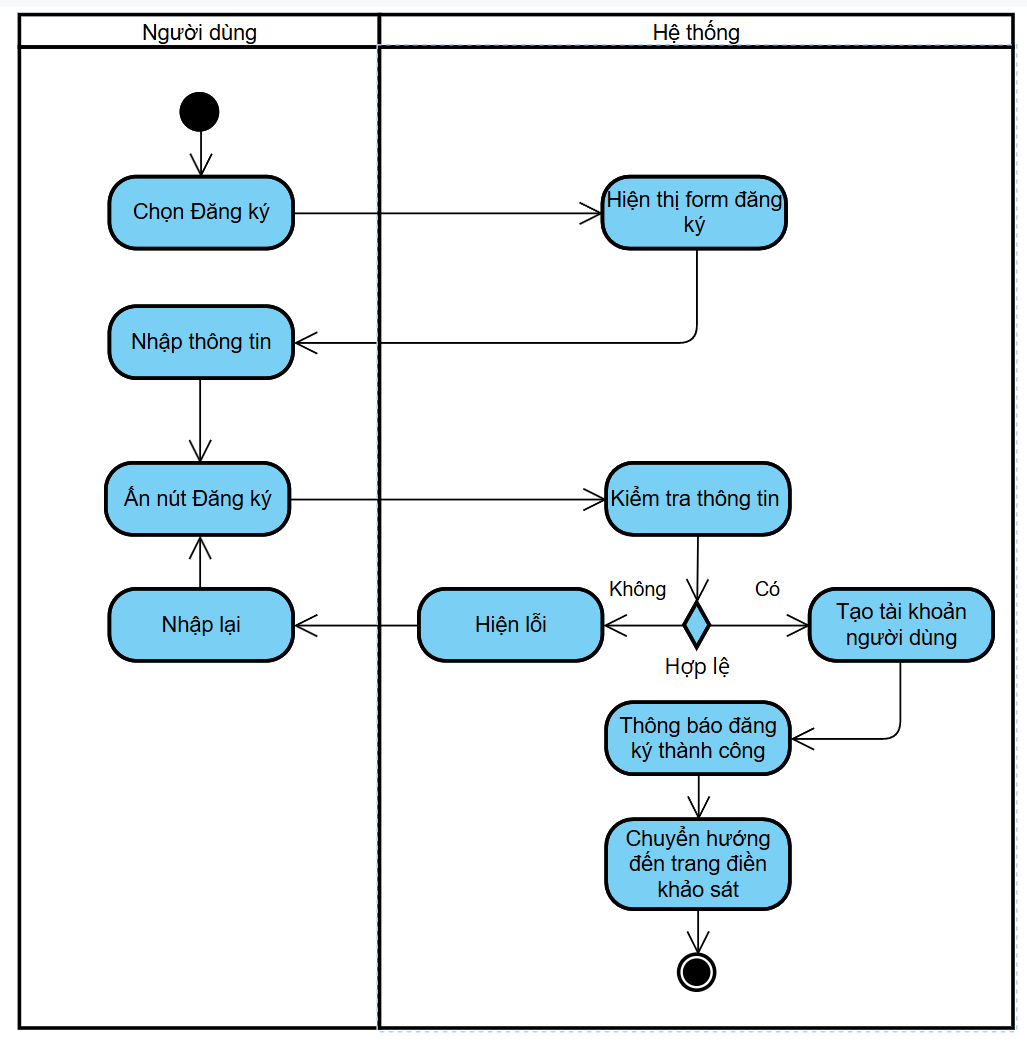
\includegraphics[width=0.5\linewidth]{figures/c3/3-3-1-ad.png} 
    & 
    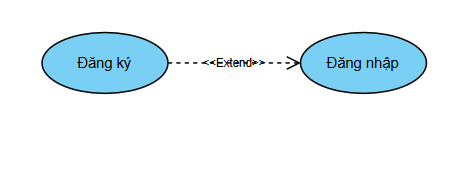
\includegraphics[width=0.45\linewidth]{figures/c3/3-3-1-rd.png} \\ 
    \hline
\end{tabular}

% \begin{figure}[H]
%     \centering  
%     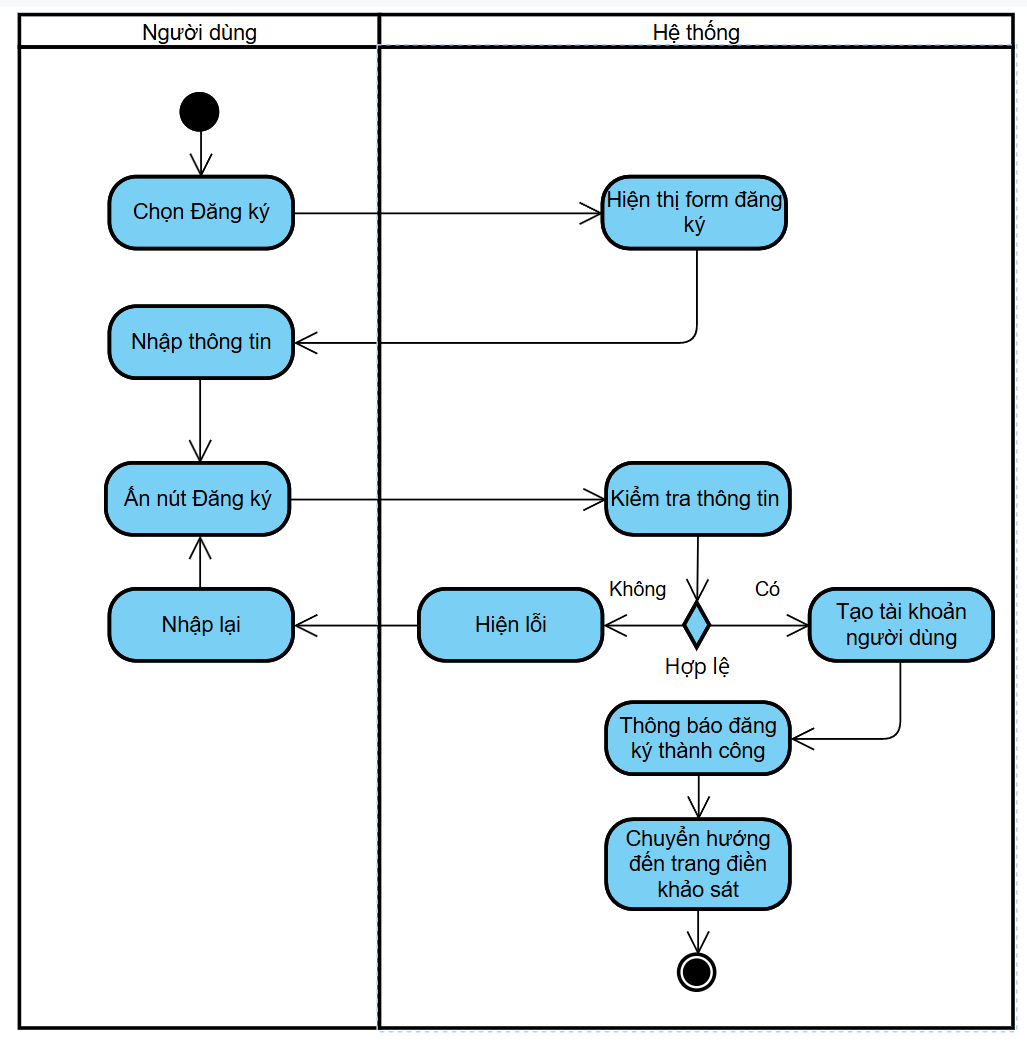
\includegraphics[width=0.5\textwidth]{figures/c3/3-3-1-ad.png}
%     \caption{Biểu đồ hoạt động ca sử dụng đăng ký.}
%     \label{fig:3-3-2-activity-diagram}
% \end{figure}



\begin{figure}[H]
    \centering  
    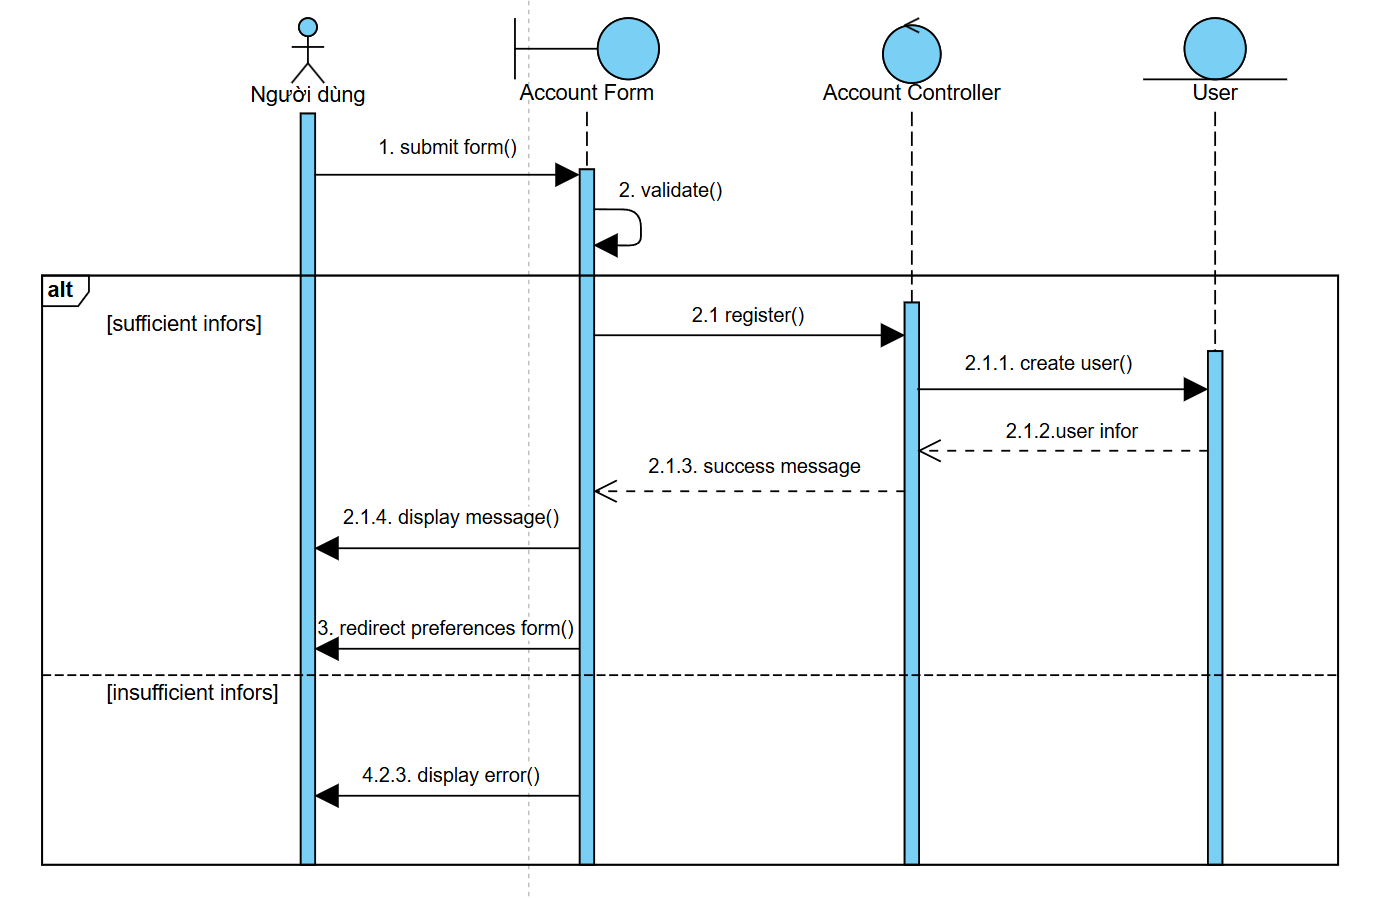
\includegraphics[width=1.05\textwidth]{figures/c3/3-3-1-sd.png}
    \caption{Biểu đồ tuần tự ca sử dụng đăng ký.}
    \label{fig:3-3-2-sequence-diagram}
\end{figure}
% \nopagebreak
% \subsection{Ca sử dụng đăng nhập}
\vspace{0.5cm}

\noindent 
\begin{tabularx}{\linewidth}{| l | X |} 
\hline 
\textbf{Mô tả} & Khi người dùng muốn sử dụng các chức năng yêu cầu quyền đăng nhập. \\ 
\hline 
\textbf{Luồng cơ bản} & 1. Truy cập trang đăng nhập \newline 
                      2. Nhập thông tin tài khoản (email / mật khẩu) \newline 
                      3. Điều hướng đến trang home - danh sách chuyến đi công khai. \\ 
\hline 
\textbf{Luồng thay thế} & - Nếu Người dùng nhập sai thông tin tài khoản hệ thống sẽ thông báo lỗi trên form đăng nhập  \newline 
                       - Người dùng có tài khoản chưa có thông tin sở thích hệ thống điều hướng đến trang khảo sát sở thích \\
\hline 
\textbf{Tiền điều kiện} & Người dùng đã đăng xuất. \\ 
\hline 
\textbf{Hậu điều kiện} & Hệ thống lưu token đăng nhập vào local trên thiết bị. \\ 
\hline 
\textbf{Yêu cầu phi chức năng} & Hệ thống xử lý đăng nhập không quá 2s. \\ 
\hline 
\end{tabularx}

\vspace{0.8cm}

\noindent 
\begin{tabular}{| c | c |}
    \hline
    \textbf{Biểu đồ hoạt động} & \textbf{Quan hệ} \\ 
    \hline
    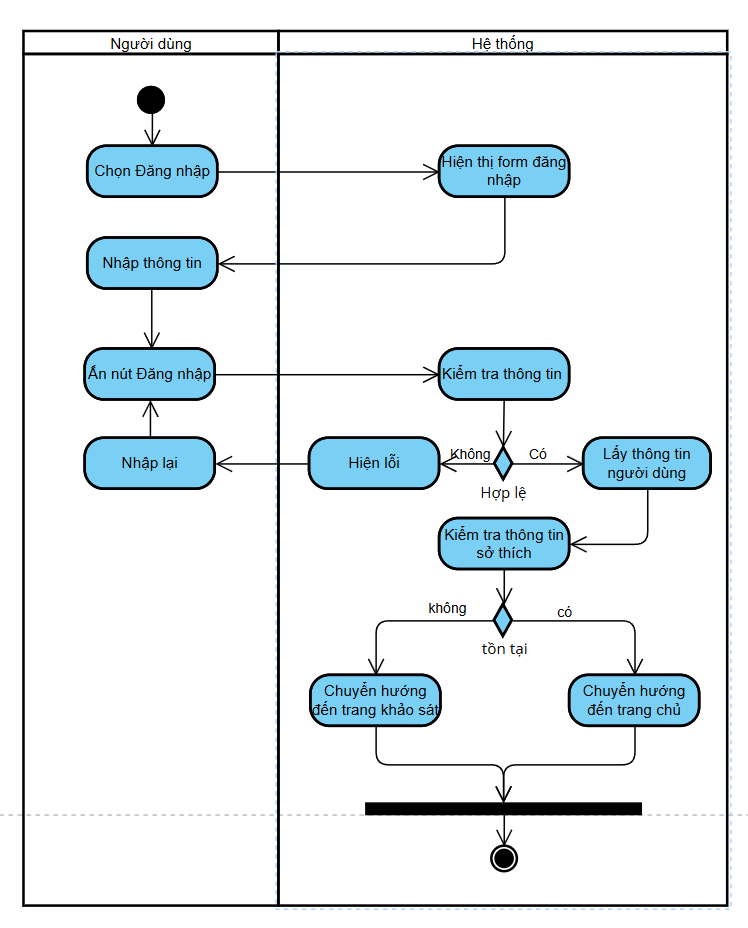
\includegraphics[width=0.5\linewidth]{figures/c3/3-3-2-ad.png} 
    & 
    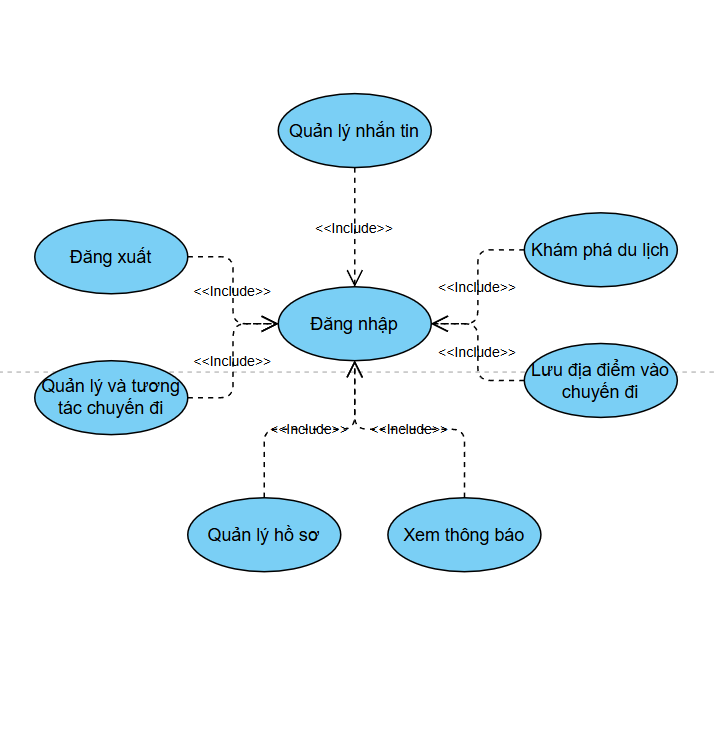
\includegraphics[width=0.45\linewidth]{figures/c3/3-3-2-rd.png} \\ 
    \hline
\end{tabular}
\vspace{0.8cm}

\begin{figure}[H]
    \centering  
    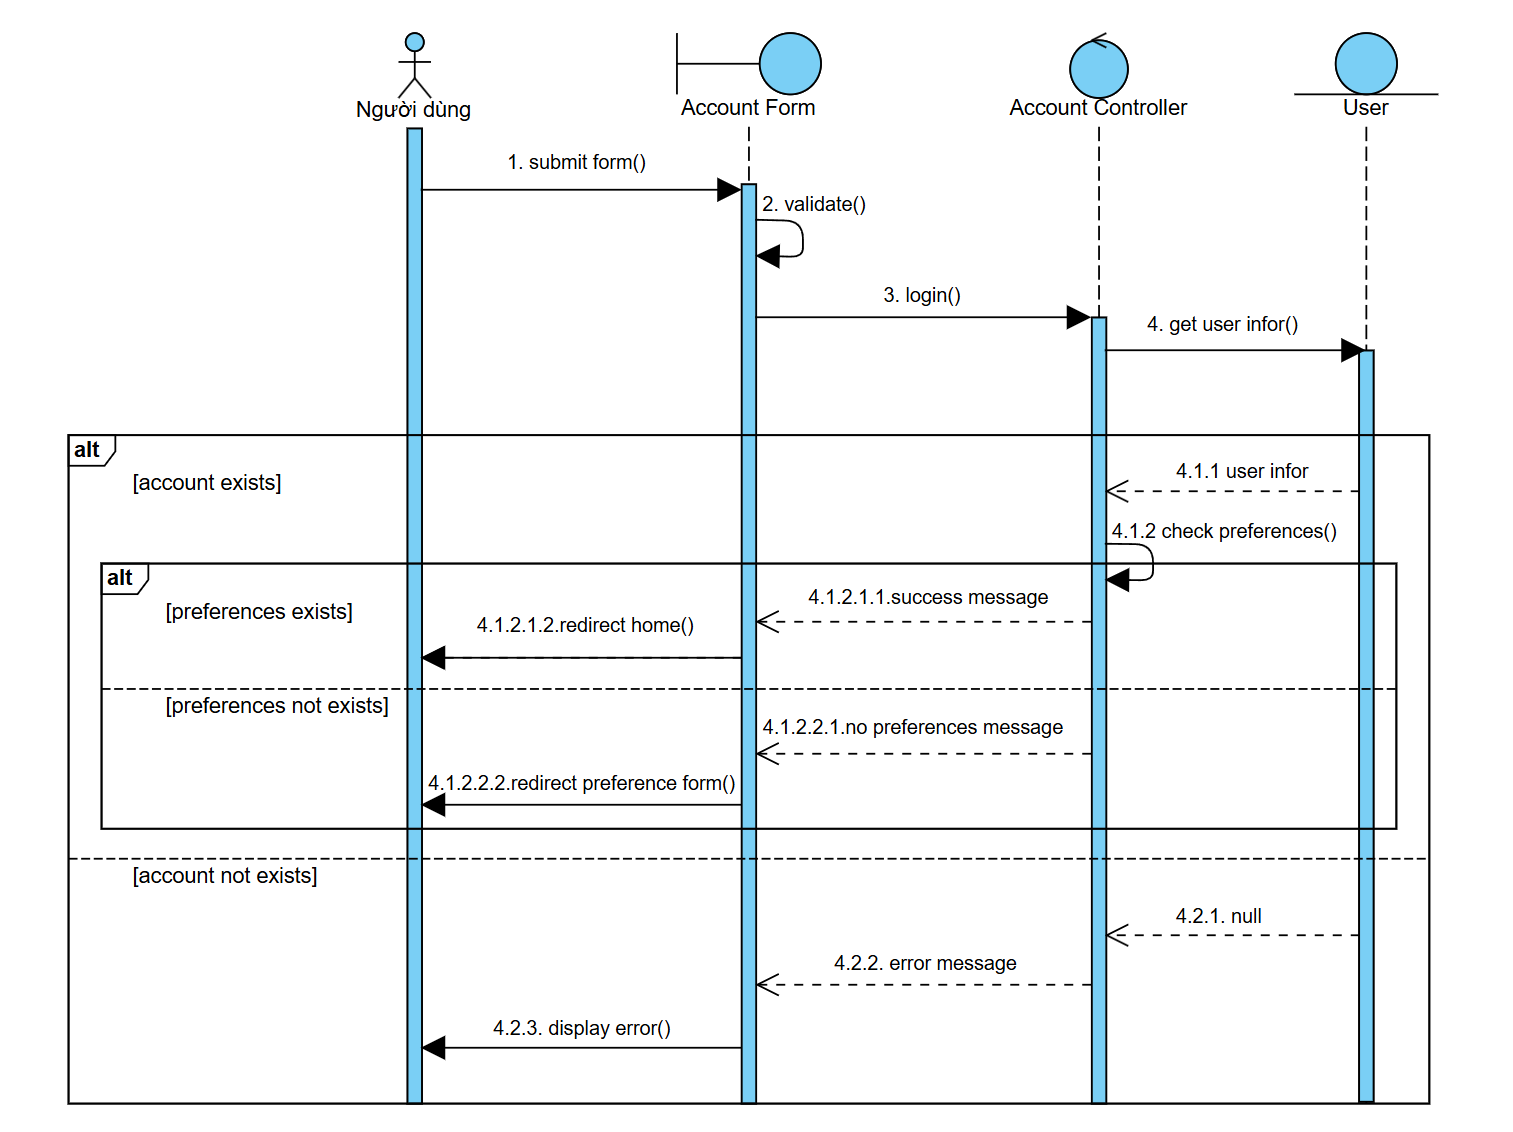
\includegraphics[width=1.05\textwidth]{figures/c3/3-3-2-sd.png}
    \caption{Biểu đồ tuần tự ca sử dụng đăng nhập.}
    \label{fig:3-3-1-sequence-diagram}
\end{figure}
% \nopagebreak
% \subsection{Ca sử dụng điền khảo sát sở thích}
\noindent Ca sử dụng này mô tả quá trình người dùng cung cấp thông tin về sở thích du lịch của mình sau khi đăng ký tài khoản. Thông tin này sẽ được hệ thống sử dụng để cá nhân hóa các gợi ý và trải nghiệm trong ứng dụng. Bảng~\ref{tab:uc_survey_spec} trình bày chi tiết đặc tả ca sử dụng, bao gồm luồng sự kiện chính, các điều kiện và yêu cầu liên quan. Các biểu đồ hoạt động, quan hệ (Bảng~\ref{tab:uc_survey_diagrams}) và tuần tự (Hình~\ref{fig:3-3-3-sequence-diagram}) minh họa rõ hơn về quy trình và tương tác hệ thống.

\begin{longtable}{| p{4cm} | p{\dimexpr\linewidth-4cm-4\tabcolsep} |} % Adjust widths as needed
    \caption{Đặc tả ca sử dụng điền khảo sát sở thích.} % Caption inside longtable
    \label{tab:uc_survey_spec} \\ % Label after caption

    \hline
    \textbf{Mô tả} & Người dùng cập nhật thông tin về sở thích du lịch của bản thân để sử dụng dịch vụ gợi ý trong ứng dụng \\
    \hline
    \endfirsthead % Header for the first page

    \hline
 
    \textbf{Mô tả} & Người dùng cập nhật thông tin về sở thích du lịch của bản thân để sử dụng dịch vụ gợi ý trong ứng dụng. \\
    \hline
    \endhead

    \hline 
    \endfoot

    \hline % Footer for the last page
    \endlastfoot

    \textbf{Luồng cơ bản} & 1. Người dùng đăng ký tài khoản mới \newline
                           2. Ứng dụng hiển thị các form lựa chọn lần lượt theo loại hình du lịch, giá tiền,v.v. \newline
                           3. Người dùng chọn các loại hình du lịch theo sở thích. \newline
                           4. Người dùng chọn khoảng giá du lịch phù hợp với bản thân. \newline
                           5. Người dùng nhấn nút hoàn tất để hoàn thành quá trình. \newline
                           6. Hệ thống điều hướng người dùng đến trang chủ của ứng dụng. \\
    \hline
    \textbf{Tiền điều kiện} & Người dùng đăng ký tài khoản thành công và chưa hoàn thành điền khảo sát sở thích. \\
    \hline
    \textbf{Hậu điều kiện} & Thông tin sở thích được lưu lại trong cơ sở dữ liệu. \\
    \hline
    \textbf{Yêu cầu phi chức năng} & Hệ thống xử lý cập nhật không quá 1s \\

\end{longtable}

\begin{table}[H] % Add table environment
    \centering
    \caption{Biểu đồ hoạt động và quan hệ ca sử dụng điền khảo sát sở thích} % Add caption
    \label{tab:uc_survey_diagrams} % Add label
    \begin{tabular}{| c | c |}
        \hline
        \textbf{Biểu đồ hoạt động} & \textbf{Quan hệ} \\
        \hline
        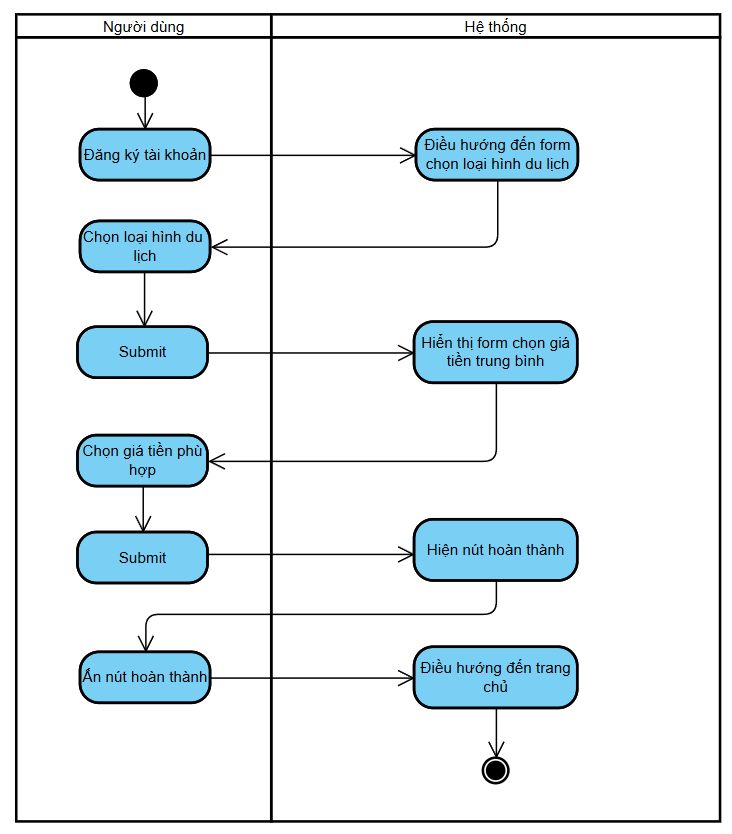
\includegraphics[width=0.5\linewidth]{figures/c3/3-3-3-ad.png}
        &
        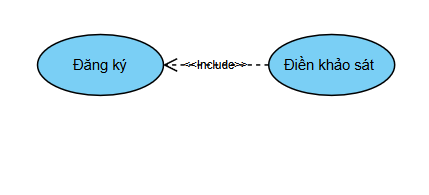
\includegraphics[width=0.45\linewidth]{figures/c3/3-3-3-rd.png} \\
        \hline
    \end{tabular}
\end{table}


\begin{figure}[H]
    \centering
    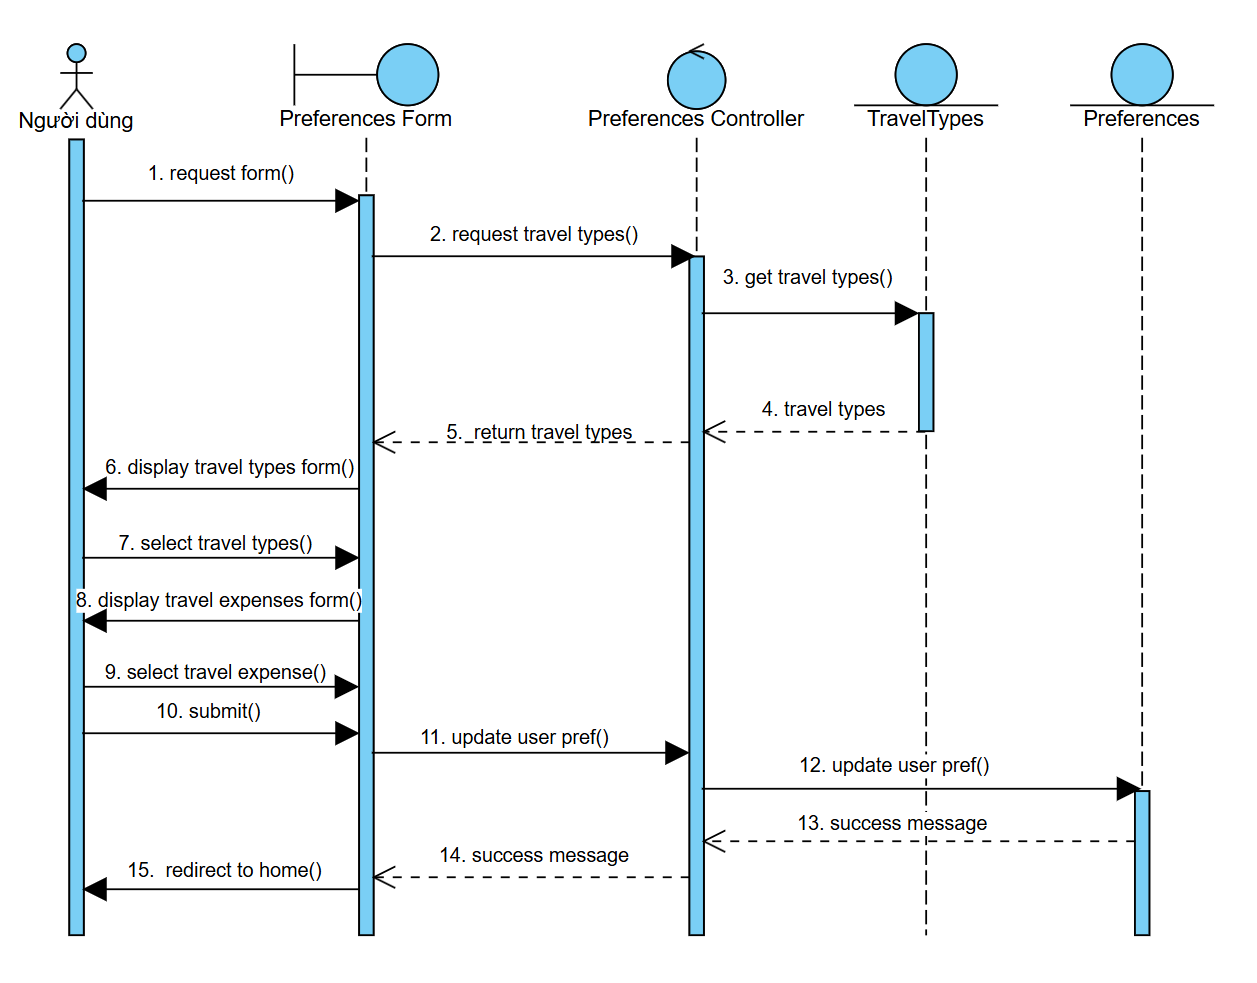
\includegraphics[width=0.85\textwidth]{figures/c3/3-3-3-sd.png}
    \caption{Biểu đồ tuần tự ca sử dụng điền khảo sát sở thích.}
    \label{fig:3-3-3-sequence-diagram}
\end{figure}
% \nopagebreak
% \subsection{Ca sử dụng chỉnh sửa thông tin cá nhân}
\vspace{0.5cm}


\noindent 
\begin{tabularx}{\linewidth}{| l | X |} 
\hline 
\textbf{Mô tả} & Người dùng cập nhật thông tin cá nhân như
địa chỉ, tên, số điện thoại, mô tả, ảnh đại diện,v.v. \\ 
\hline 
\textbf{Luồng cơ bản} & 1. Người dùng truy cập tab tài khoản và bấm vào trang hồ sơ của bản thân \newline
                       2. Người dùng ấn vào nút chính sửa \newline
                       3. Người dùng nhập các thông tin cần thay đổi. \newline
                       5. Người dùng ấn nút submit. \newline
                       6. Hệ thống cập nhật thông tin người dùng và thông báo cập nhật thành công. \\
\hline 
\textbf{Luồng thay thế} & Nếu Người dùng nhập thông tin không hợp lệ hệ thống sẽ báo lỗi. \\
\hline 
\textbf{Tiền điều kiện} & Người dùng đang đăng nhập và phiên đăng nhập chưa kết thúc. \\
\hline 
\textbf{Hậu điều kiện} & Thông tin mới của người dùng được cập nhật. \\

\hline 
\textbf{Yêu cầu phi chức năng} & Hệ thống xử lý cập nhật không quá 5s (do có upload ảnh) \\ 
\hline 
\end{tabularx}

\vspace{0.8cm}

\noindent 
\begin{tabular}{| c | c |}
    \hline
    \textbf{Biểu đồ hoạt động} & \textbf{Quan hệ} \\ 
    \hline
    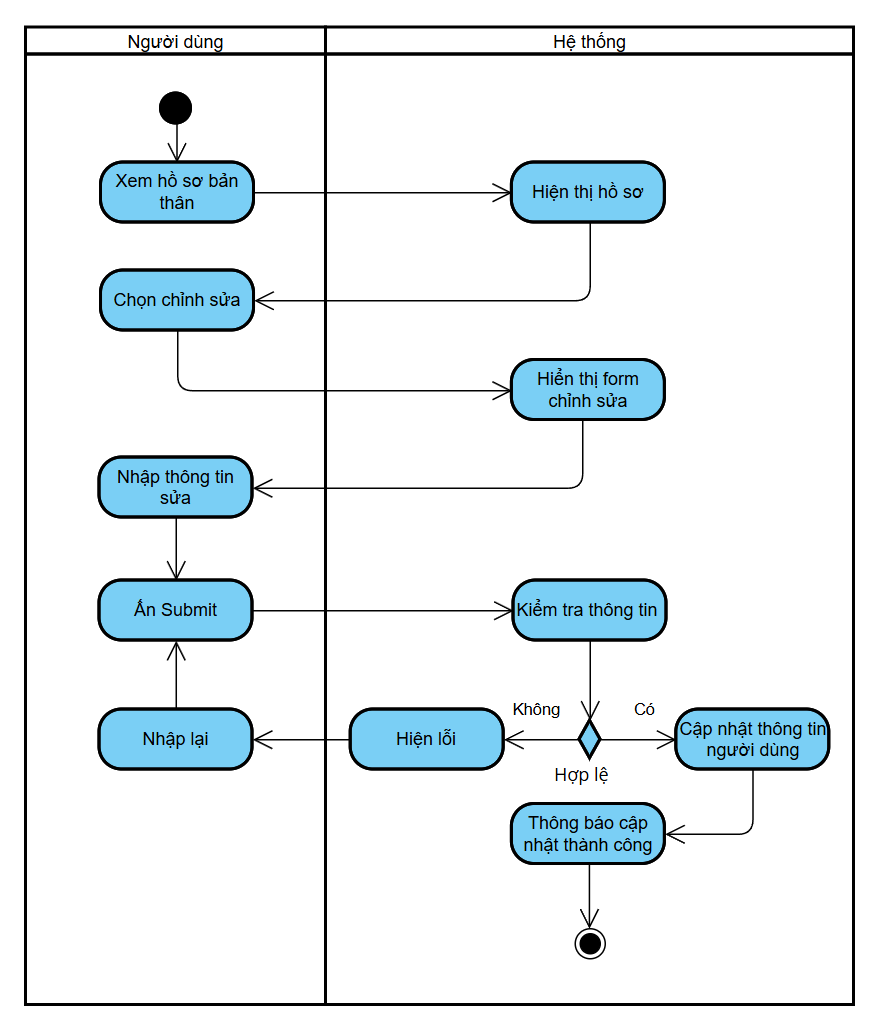
\includegraphics[width=0.5\linewidth]{figures/c3/3-3-4-ad.png} 
    & 
    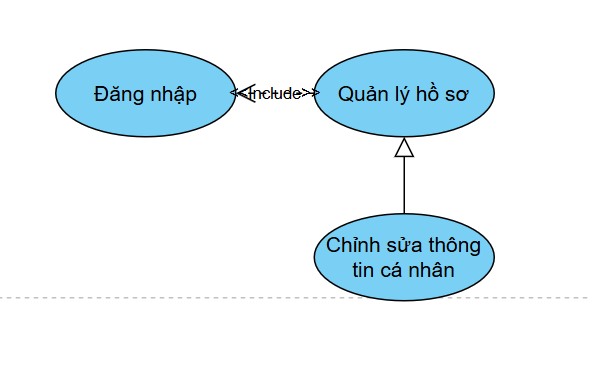
\includegraphics[width=0.45\linewidth]{figures/c3/3-3-4-rd.png} \\ 
    \hline
\end{tabular}



\begin{figure}[H]
    \centering  
    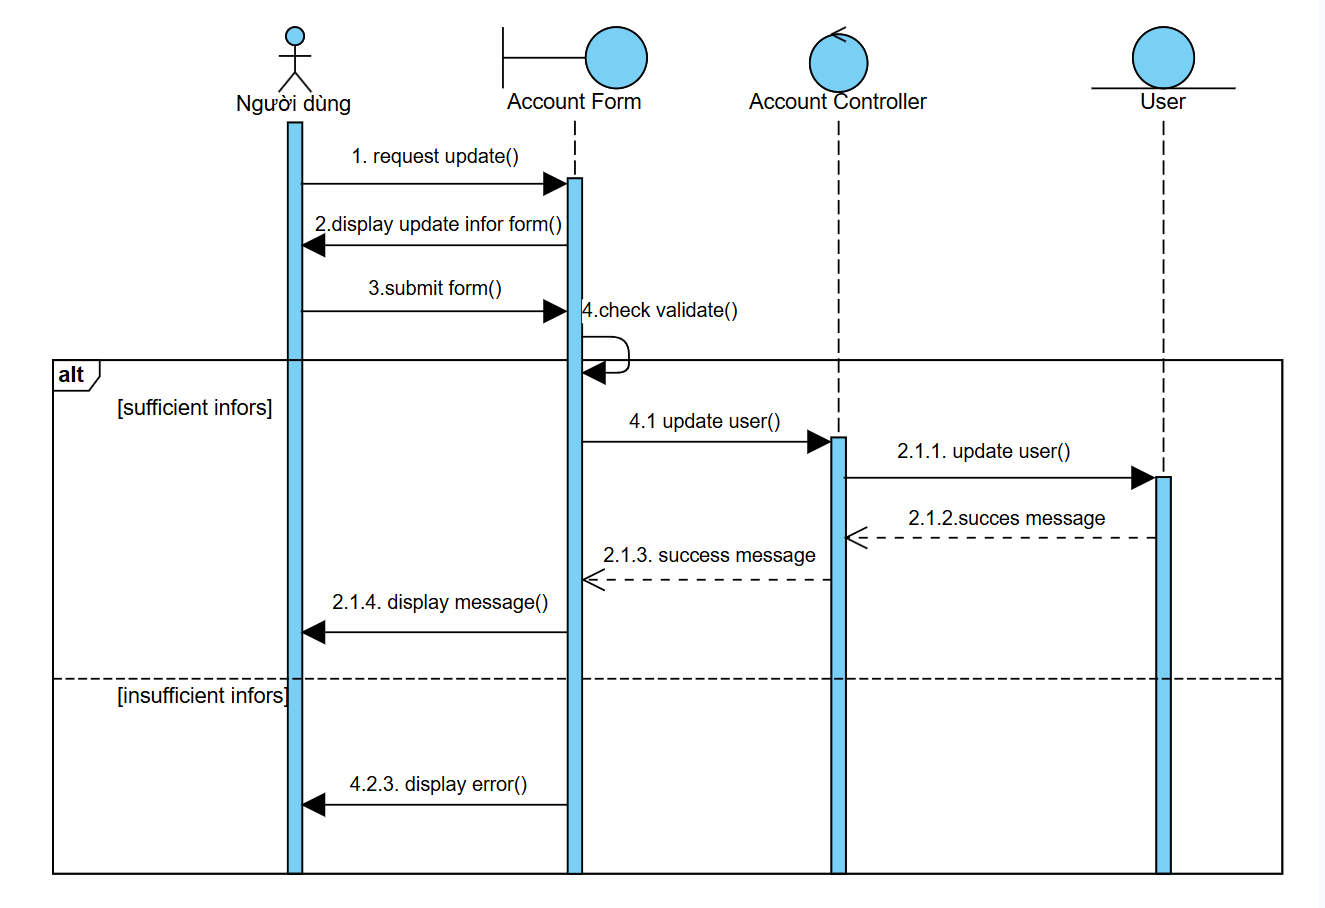
\includegraphics[width=1\textwidth]{figures/c3/3-3-4-sd.png}
    \caption{Biểu đồ tuần tự ca sử dụng chỉnh sửa thông tin cá nhân.}
    \label{fig:3-3-4-sequence-diagram}
\end{figure}
% \nopagebreak
\subsection{Ca sử dụng tra cứu du lịch}
\noindent Ca sử dụng này mô tả quá trình người dùng tìm kiếm thông tin về các địa điểm du lịch, sự kiện, hoặc các dịch vụ khác thông qua chức năng tìm kiếm của ứng dụng. Người dùng có thể nhập từ khóa và áp dụng các bộ lọc để thu hẹp kết quả. Bảng~\ref{tab:uc_search_spec} trình bày chi tiết đặc tả ca sử dụng, bao gồm luồng sự kiện chính, các điều kiện và yêu cầu liên quan. Các biểu đồ hoạt động, quan hệ (Bảng~\ref{tab:uc_search_diagrams}) và tuần tự (Hình~\ref{fig:3-3-5-sequence-diagram}) minh họa rõ hơn về quy trình và tương tác hệ thống khi người dùng thực hiện tra cứu.
% \vspace{0.5cm} % Adjust spacing if needed

% Use longtable environment
% Need \usepackage{longtable} and \usepackage{calc} in preamble
\begin{longtable}{| p{4cm} | p{\dimexpr\linewidth-4cm-4\tabcolsep} |} % Adjust widths as needed
    \caption{Đặc tả ca sử dụng tra cứu du lịch} % Caption inside longtable
    \label{tab:uc_search_spec} \\ % Label after caption

    \hline
    \textbf{Mô tả} & Người dùng tra cứu và lọc tên địa điểm du lịch, sự kiện, điểm đến muốn tìm hiểu. \\
    \hline
    \endfirsthead % Header for the first page

    \hline
    % \multicolumn{2}{|c|}{(Tiếp theo)} \\ % Header for subsequent pages
    % \hline
    \textbf{Mô tả} & Người dùng tra cứu và lọc tên địa điểm du lịch, sự kiện, điểm đến muốn tìm hiểu. \\
    \hline
    \endhead

    \hline 
    % \multicolumn{2}{|r|}{{Tiếp tục ở trang sau}} \\ % Footer for pages before the last
    \endfoot

    \hline % Footer for the last page
    \endlastfoot

    % --- Table Content ---
    \textbf{Luồng cơ bản} & 1. Người dùng truy cập tab khám phá và bấm vào thanh tìm kiếm. \newline
                           2. Hệ thống hiển thị lịch sử tìm kiếm và các bộ lọc. \newline
                           3. Người dùng nhập từ khóa tìm kiếm. \newline
                           4. Người dùng chọn bộ lọc (sự kiện, địa điểm, nhà hàng, khách sạn, điểm đến, v.v.). \newline
                           5. Hệ thống tra cứu, lưu từ khóa tìm kiếm và hiển thị kết quả theo danh sách. \\
    \hline
    % \textbf{Luồng thay thế} & (Nếu có luồng thay thế, thêm vào đây) \\
    % \hline
    \textbf{Tiền điều kiện} & Người dùng đang đăng nhập và phiên đăng nhập chưa kết thúc. \\
    \hline
    \textbf{Hậu điều kiện} & - Người dùng có thể xem thông tin về các kết quả tìm kiếm.\newline
                           - Hệ thống lưu lại lịch sử tìm kiếm của người dùng. \newline
                           - Hệ thống có thể cập nhật sở thích của người dùng dựa trên từ khóa tìm kiếm. \\
    \hline
    \textbf{Yêu cầu phi chức năng} & Hệ thống xử lý tìm kiếm không quá 2 giây. \\
    % --- End Table Content ---

\end{longtable}
% \vspace{0.8cm}

\begin{table}[H] % Wrap the diagrams table
    \centering
    \caption{Biểu đồ hoạt động và quan hệ ca sử dụng tra cứu du lịch} % Add caption
    \label{tab:uc_search_diagrams} % Add label
    \begin{tabular}{| c | c |}
        \hline
        \textbf{Biểu đồ hoạt động} & \textbf{Quan hệ} \\
        \hline
        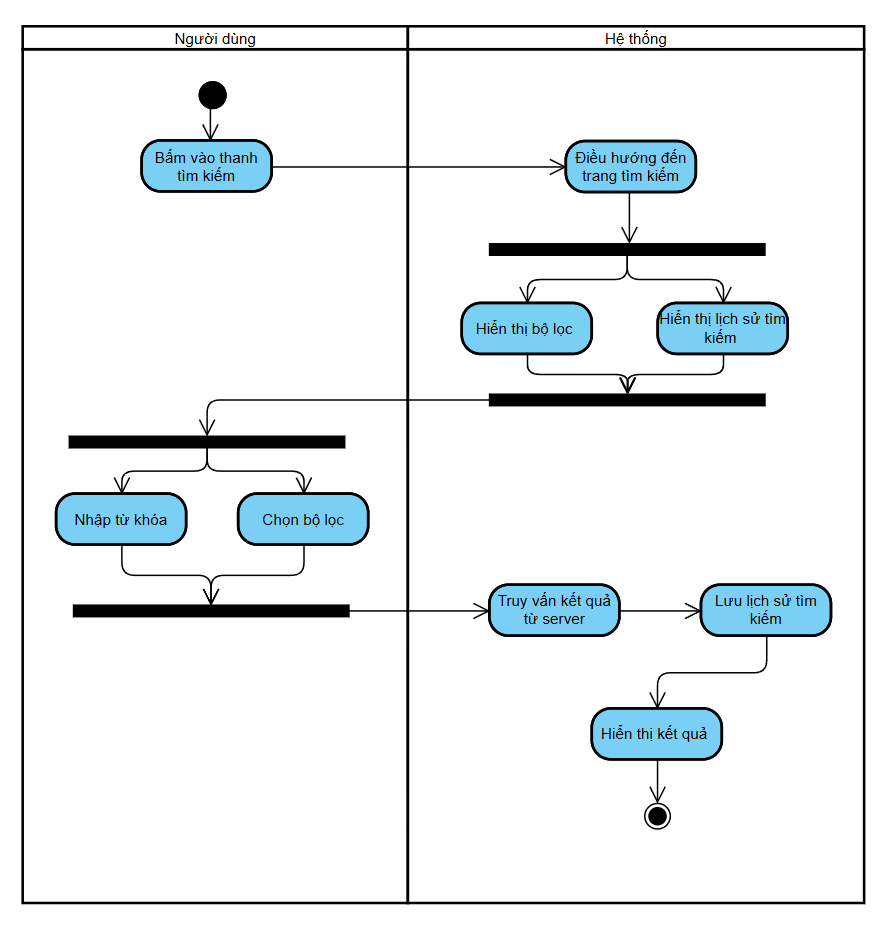
\includegraphics[width=0.5\linewidth]{figures/c3/3-3-5-ad.png}
        &
        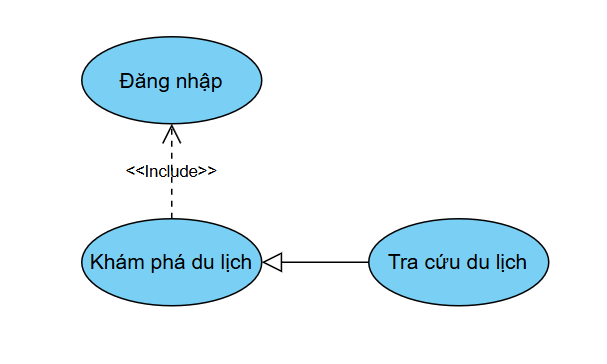
\includegraphics[width=0.45\linewidth]{figures/c3/3-3-5-rd.png} \\
        \hline
    \end{tabular}
\end{table}

\begin{figure}[H]
    \centering
    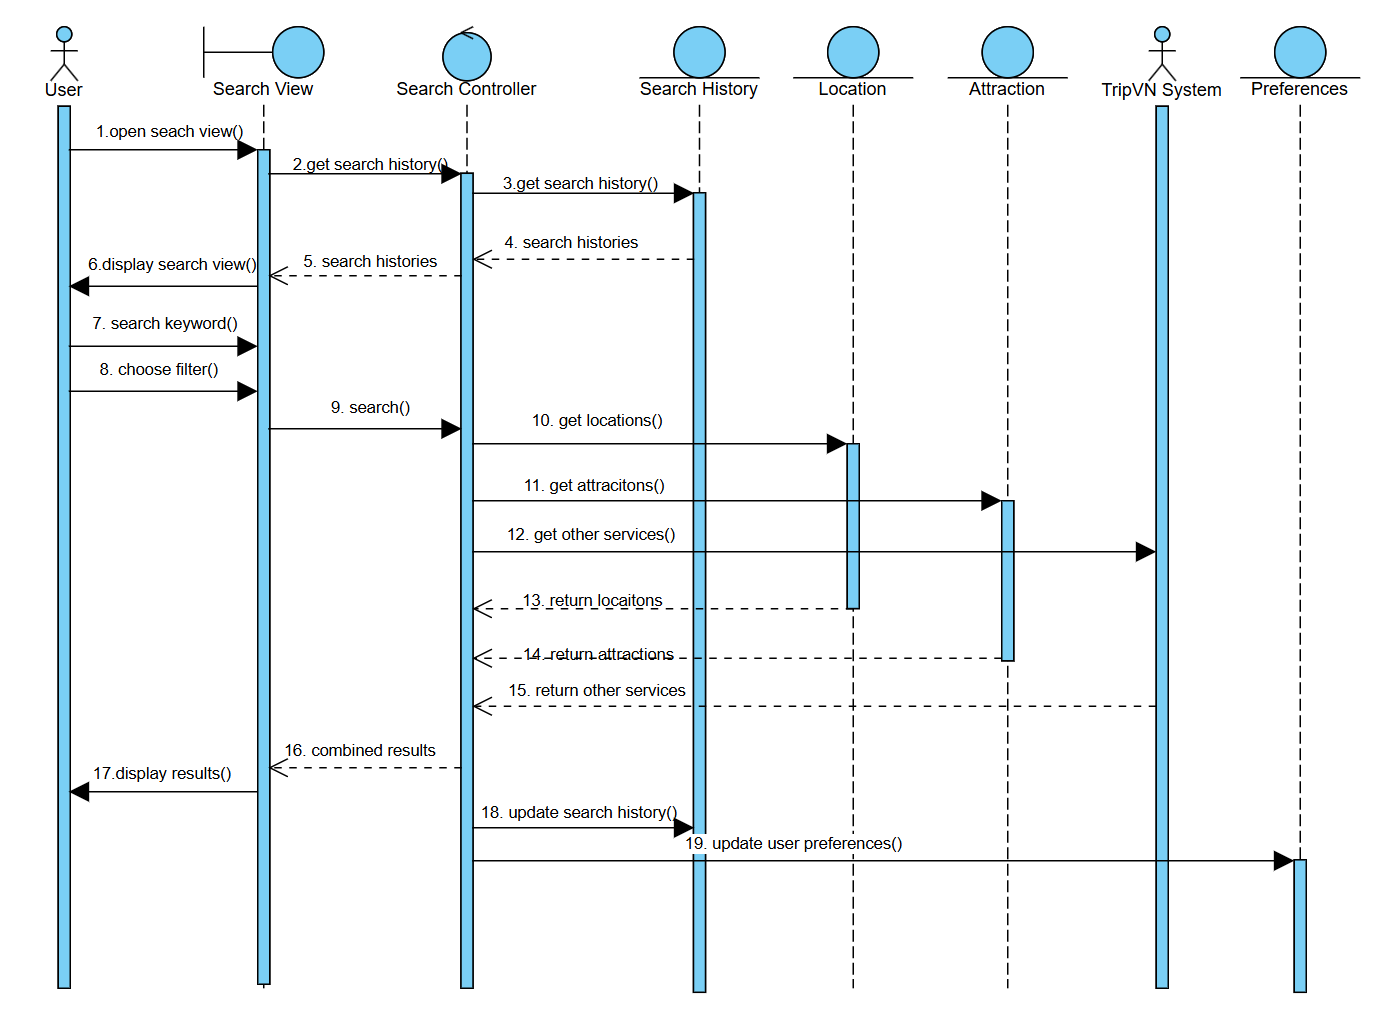
\includegraphics[width=1\textwidth]{figures/c3/3-3-5-sd.png} % Adjusted width slightly
    \caption{Biểu đồ tuần tự ca sử dụng tra cứu du lịch.}
    \label{fig:3-3-5-sequence-diagram}
\end{figure}
\nopagebreak
\subsection{Ca sử dụng xem danh sách địa điểm được gợi ý}
\noindent Ca sử dụng này mô tả cách người dùng xem danh sách các địa điểm du lịch được hệ thống gợi ý dựa trên sở thích cá nhân. Người dùng cũng có thể tùy chỉnh các bộ lọc sở thích để nhận được những gợi ý khác phù hợp hơn. Bảng~\ref{tab:uc_view_recommendations_spec} trình bày chi tiết đặc tả ca sử dụng, bao gồm luồng sự kiện chính, luồng thay thế, các điều kiện và yêu cầu liên quan. Các biểu đồ hoạt động, quan hệ (Bảng~\ref{tab:uc_view_recommendations_diagrams}) và tuần tự (Hình~\ref{fig:3-3-6-sequence-diagram}) minh họa rõ hơn về quy trình và tương tác hệ thống khi người dùng xem các gợi ý.
% \vspace{0.5cm} % Adjust spacing if needed

% Use longtable environment
% Need \usepackage{longtable} and \usepackage{calc} in preamble
\begin{longtable}{| p{4cm} | p{\dimexpr\linewidth-4cm-4\tabcolsep} |} % Adjust widths as needed
    \caption{Đặc tả ca sử dụng xem danh sách địa điểm được gợi ý} % Caption inside longtable
    \label{tab:uc_view_recommendations_spec} \\ % Label after caption

    \hline
    \textbf{Mô tả} & Người dùng xem danh sách địa điểm du lịch gợi ý cho bản thân và tùy chỉnh sở thích về loại hình du lịch để lấy gợi ý khác. \\
    \hline
    \endfirsthead % Header for the first page

    % No \endhead content needed

    % No \endfoot content needed

    \hline % Footer for the last page
    \endlastfoot

    % --- Table Content ---
    \textbf{Luồng cơ bản} & 1. Người dùng truy cập tab khám phá. \newline
                           2. Người dùng bấm vào trang đề xuất địa điểm du lịch. \newline
                           3. Hệ thống điều hướng đến trang hiển thị danh sách địa điểm du lịch gợi ý cho người dùng và bộ lọc tùy chỉnh. \\
    \hline
    \textbf{Luồng thay thế} & Người dùng tùy chỉnh bộ lọc sở thích loại hình du lịch để nhận gợi ý khác. \\
    \hline
    \textbf{Tiền điều kiện} & - Người dùng đang đăng nhập và phiên đăng nhập chưa kết thúc. \newline
                             - Người dùng có thông tin về sở thích. \\
    \hline
    \textbf{Hậu điều kiện} & - Người dùng có thể chọn địa điểm trong danh sách để xem chi tiết. \\
    \hline
    \textbf{Yêu cầu phi chức năng} & Hệ thống xử lý lấy danh sách không quá 2s. \\
    % --- End Table Content ---

\end{longtable}
\vspace{0.8cm}

\begin{table}[H] % Wrap the diagrams table
    \centering
    \caption{Biểu đồ hoạt động ca sử dụng xem danh sách địa điểm được gợi ý} % Add caption
    \label{tab:uc_view_recommendations_diagrams} % Add label
    \begin{tabular}{| c | c |}
        \hline
        \textbf{Biểu đồ hoạt động} & \textbf{Quan hệ} \\
        \hline
        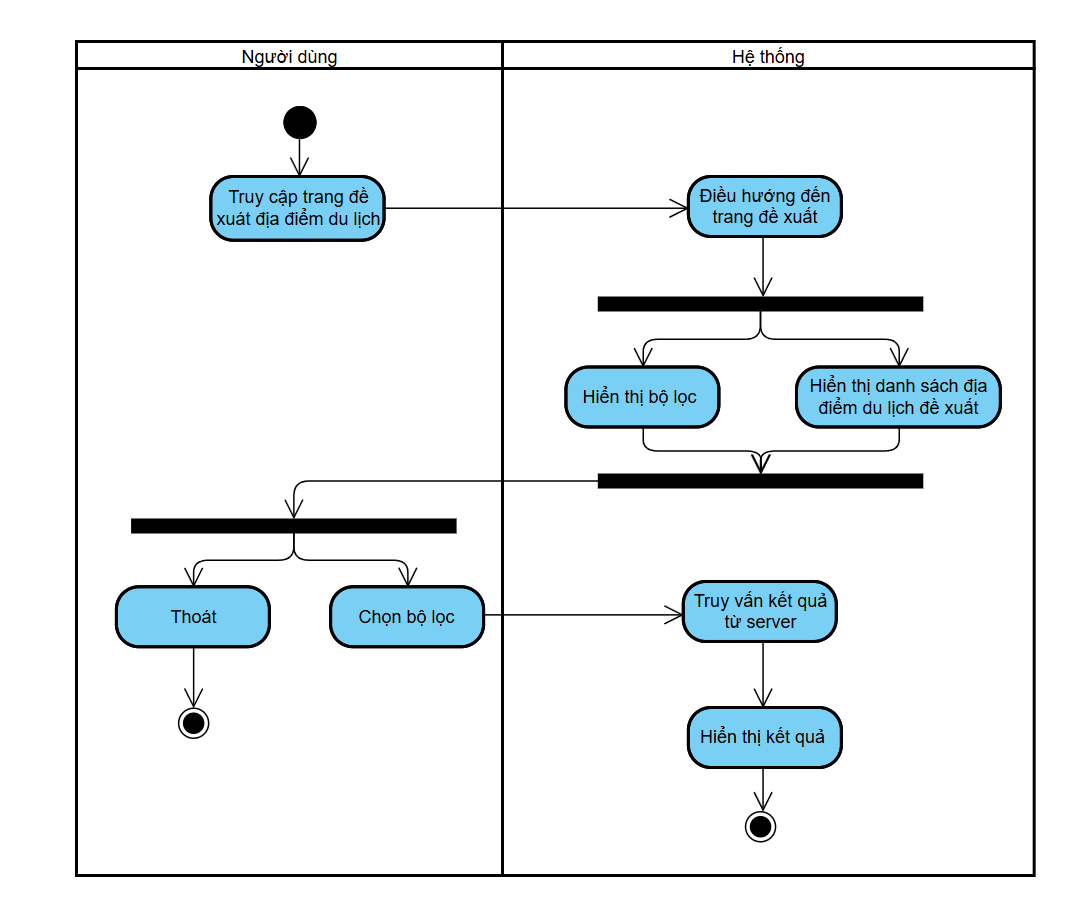
\includegraphics[width=0.5\linewidth]{figures/c3/3-3-6-ad.png}
        &
        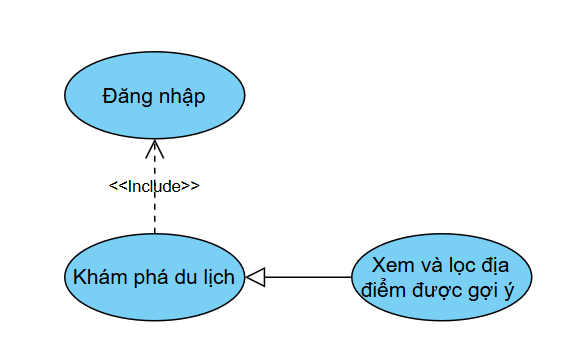
\includegraphics[width=0.45\linewidth]{figures/c3/3-3-6-rd.png} \\
        \hline
    \end{tabular}
\end{table}

\begin{figure}[H]
    \centering
    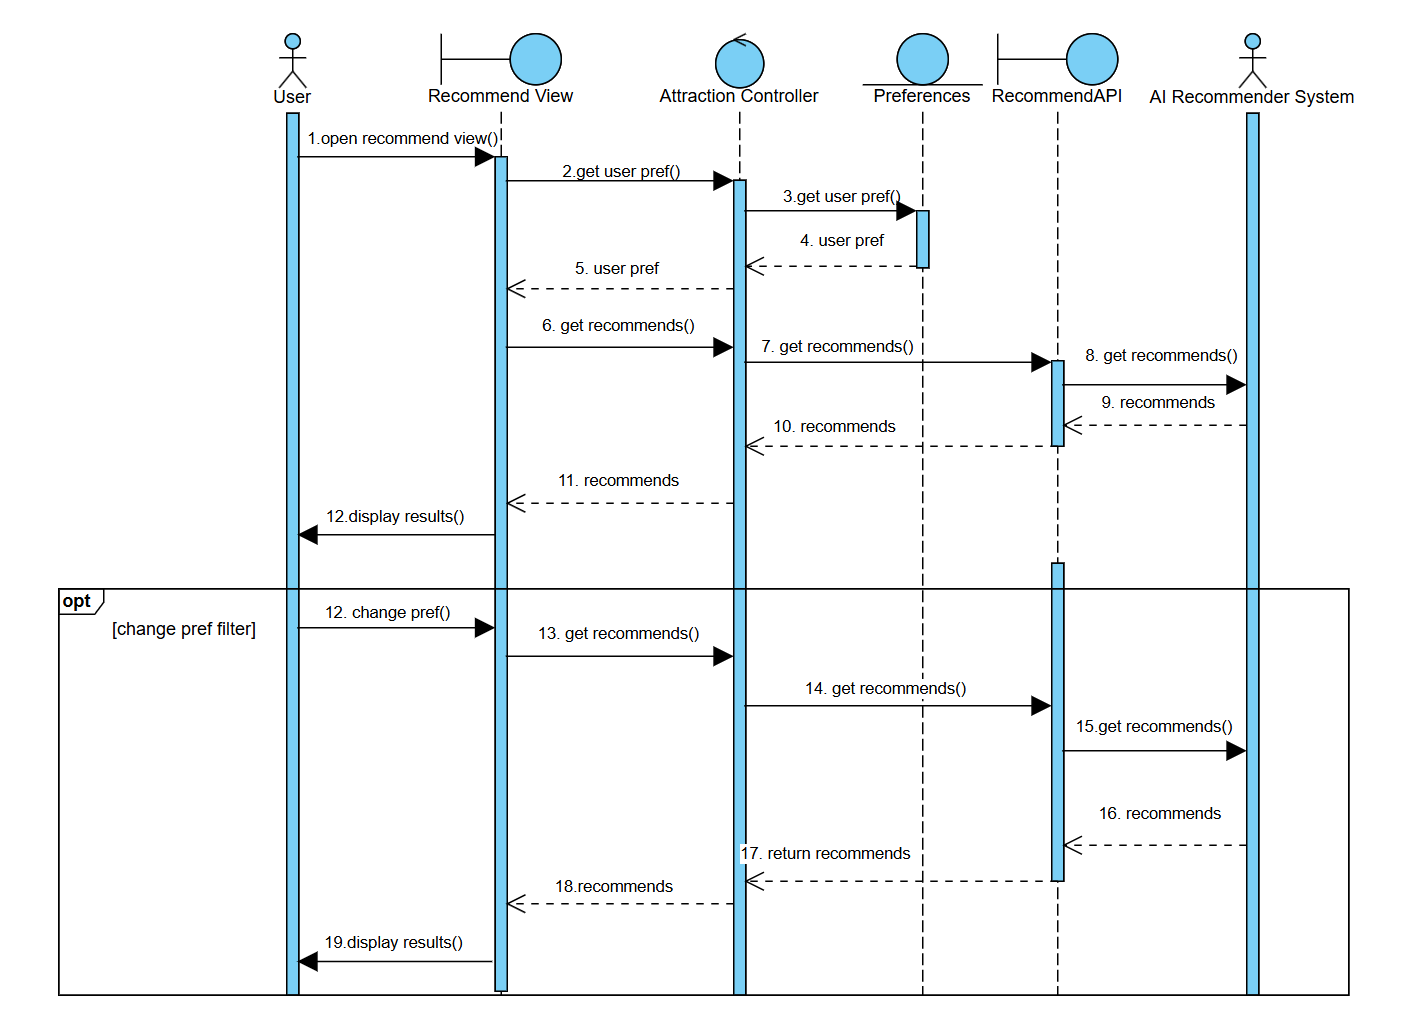
\includegraphics[width=1\textwidth]{figures/c3/3-3-6-sd.png} % Adjusted width slightly
    \caption{Biểu đồ tuần tự ca sử dụng xem danh sách địa điểm được gợi ý.}
    \label{fig:3-3-6-sequence-diagram}
\end{figure}
\nopagebreak
\subsection{Ca sử dụng xem danh sách địa điểm gần người dùng}
\noindent Ca sử dụng này mô tả cách người dùng tìm kiếm và xem danh sách các địa điểm (du lịch, nhà hàng, khách sạn) ở gần vị trí hiện tại của họ. Hệ thống yêu cầu quyền truy cập vị trí để thực hiện chức năng này. Bảng~\ref{tab:uc_nearby_places_spec} trình bày chi tiết đặc tả ca sử dụng, bao gồm luồng sự kiện chính, luồng thay thế, các điều kiện và yêu cầu liên quan. Các biểu đồ hoạt động, quan hệ (Bảng~\ref{tab:uc_nearby_places_diagrams}) và tuần tự (Hình~\ref{fig:3-3-7-sequence-diagram}) minh họa rõ hơn về quy trình và tương tác hệ thống.
% \vspace{0.5cm} % Adjust spacing if needed

% Use longtable environment
% Need \usepackage{longtable} and \usepackage{calc} in preamble
\begin{longtable}{| p{4cm} | p{\dimexpr\linewidth-4cm-4\tabcolsep} |} % Adjust widths as needed
    \caption{Đặc tả ca sử dụng xem danh sách địa điểm gần người dùng} % Caption inside longtable
    \label{tab:uc_nearby_places_spec} \\ % Label after caption

    \hline
    \textbf{Mô tả} & Người dùng xem danh sách địa điểm du lịch, nhà hàng, khách sạn gần bản thân. \\
    \hline
    \endfirsthead % Header for the first page

    % No \endhead content needed

    % No \endfoot content needed

    \hline % Footer for the last page
    \endlastfoot

    % --- Table Content ---
    \textbf{Luồng cơ bản} & 1. Người dùng truy cập tab khám phá và bấm vào thanh tìm kiếm. \newline
                           2. Người dùng bấm vào biểu tượng ``Lân cận". \newline
                           3. Hệ thống hiển thị hộp thoại cấp quyền thông tin vị trí hiện tại. \newline
                           4. Người dùng cấp quyền cho hệ thống. \newline
                           5. Hệ thống lấy vị trí hiện tại của người dùng và hiển thị danh sách địa điểm gần nhất. \\
    \hline
    \textbf{Luồng thay thế} & Người dùng không cấp quyền truy cập vị trí sẽ nhận thông báo lỗi. \\
    \hline
    \textbf{Tiền điều kiện} & Người dùng đang đăng nhập và phiên đăng nhập chưa kết thúc. \\
    \hline
    \textbf{Hậu điều kiện} & - Người dùng có thể xem địa chỉ của bản thân và xem chi tiết các dịch vụ, địa điểm trong danh sách. \newline
                           - Người dùng có thể xem dạng bản đồ các địa điểm trong danh sách. \\
    \hline
    \textbf{Yêu cầu phi chức năng} & Hệ thống xử lý lấy danh sách không quá 5s. \\
    % --- End Table Content ---

\end{longtable}
\vspace{0.8cm}

\begin{table}[H] % Wrap the diagrams table
    \centering
    \caption{Biểu đồ hoạt động ca sử dụng xem danh sách địa điểm gần người dùng} % Add caption
    \label{tab:uc_nearby_places_diagrams} % Add label
    \begin{tabular}{| c | c |}
        \hline
        \textbf{Biểu đồ hoạt động} & \textbf{Quan hệ} \\
        \hline
        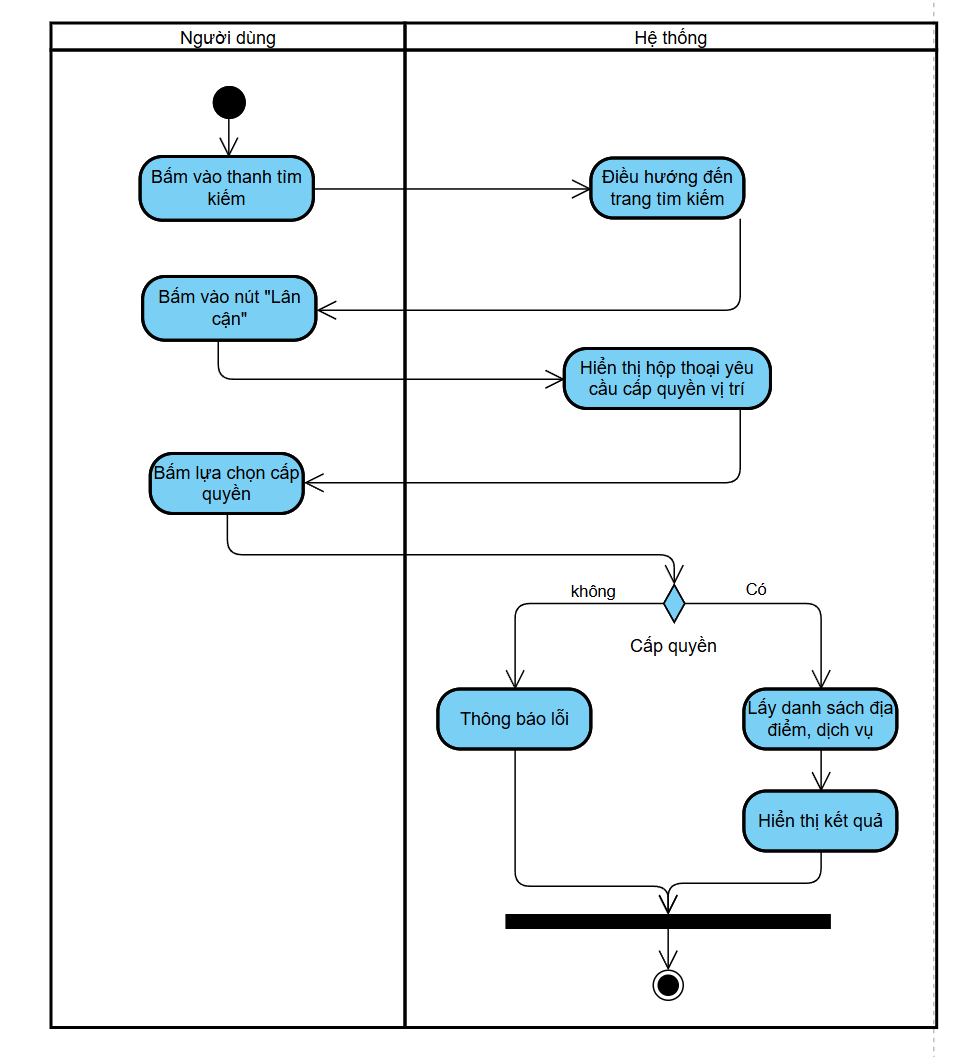
\includegraphics[width=0.5\linewidth]{figures/c3/3-3-7-ad.png} % Specified width
        &
        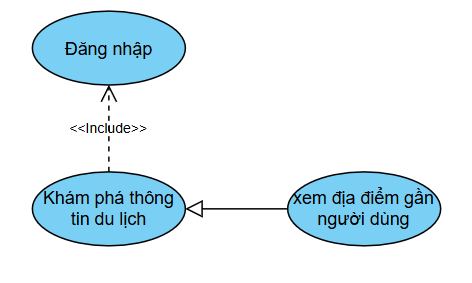
\includegraphics[width=0.45\linewidth]{figures/c3/3-3-7-rd.png} \\ % Specified width
        \hline
    \end{tabular}
\end{table}

\begin{figure}[H]
    \centering
    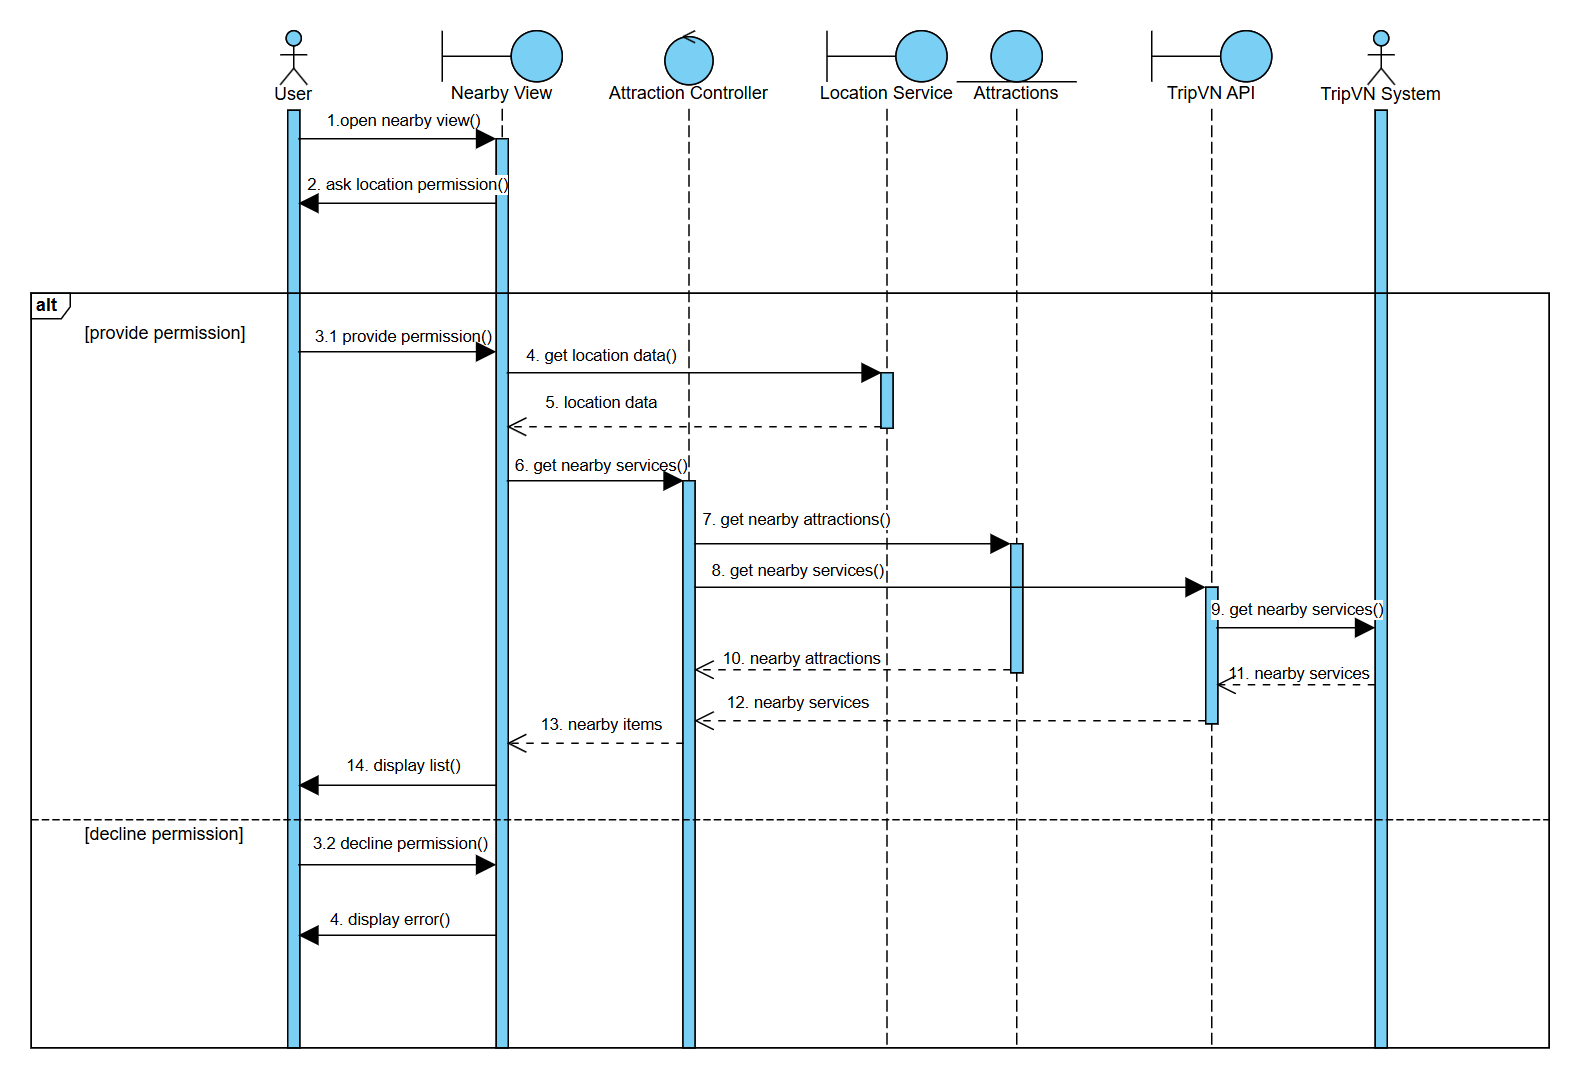
\includegraphics[width=1\textwidth]{figures/c3/3-3-7-sd.png} % Specified width
    \caption{Biểu đồ tuần tự ca sử dụng xem danh sách địa điểm gần người dùng.}
    \label{fig:3-3-7-sequence-diagram}
\end{figure}
\nopagebreak
\subsection{Ca sử dụng xem thông tin chi tiết địa điểm du lịch}
\noindent Ca sử dụng này mô tả cách người dùng xem thông tin chi tiết về một địa điểm du lịch cụ thể, bao gồm mô tả, hình ảnh, địa chỉ, đánh giá và các địa điểm liên quan khác. Bảng~\ref{tab:uc_view_place_details_spec} trình bày chi tiết đặc tả ca sử dụng, bao gồm luồng sự kiện chính, các điều kiện và yêu cầu liên quan. Các biểu đồ hoạt động, quan hệ (Bảng~\ref{tab:uc_view_place_details_diagrams}) và tuần tự (Hình~\ref{fig:3-3-8-sequence-diagram}) minh họa rõ hơn về quy trình và tương tác hệ thống khi người dùng xem chi tiết địa điểm.
% \vspace{0.5cm} % Adjust spacing if needed

% Use longtable environment
% Need \usepackage{longtable} and \usepackage{calc} in preamble
\begin{longtable}{| p{4cm} | p{\dimexpr\linewidth-4cm-4\tabcolsep} |} % Adjust widths as needed
    \caption{Đặc tả ca sử dụng xem thông tin chi tiết địa điểm du lịch} % Caption inside longtable
    \label{tab:uc_view_place_details_spec} \\ % Label after caption

    \hline
    \textbf{Mô tả} & Người dùng xem chi tiết thông tin địa điểm du lịch. \\
    \hline
    \endfirsthead % Header for the first page

    % No \endhead content needed

    % No \endfoot content needed

    \hline % Footer for the last page
    \endlastfoot

    % --- Table Content ---
    \textbf{Luồng cơ bản} & 1. Người dùng bấm vào một địa điểm du lịch muốn xem thông tin (từ danh sách tìm kiếm, gợi ý, bản đồ, v.v.). \newline
                           2. Hệ thống lấy thông tin chi tiết của địa điểm từ cơ sở dữ liệu và các API bên ngoài (nếu cần). \newline
                           3. Hệ thống hiển thị thông tin chi tiết địa điểm du lịch bao gồm tên, mô tả, địa chỉ, số điện thoại, ảnh, đánh giá và các địa điểm liên quan. \\
    \hline
    % \textbf{Luồng thay thế} & (Nếu có luồng thay thế, ví dụ: địa điểm không tồn tại, lỗi API) \\
    % \hline
    \textbf{Tiền điều kiện} & Người dùng đang đăng nhập và phiên đăng nhập chưa kết thúc. \\
    \hline
    \textbf{Hậu điều kiện} & - Người dùng có thể xem thông tin về địa điểm như mô tả, địa chỉ, sđt, ảnh. \newline
                           - Người dùng có thể xem chi tiết các đánh giá về địa điểm. \newline
                           - Người dùng có thể xem chi tiết các địa điểm liên quan. \\
    \hline
    \textbf{Yêu cầu phi chức năng} & Hệ thống xử lý lấy và hiển thị thông tin không quá 2 giây. \\
    % --- End Table Content ---

\end{longtable}
\vspace{0.8cm}

\begin{table}[H] % Wrap the diagrams table
    \centering
    \caption{Biểu đồ hoạt động ca sử dụng xem thông tin chi tiết địa điểm du lịch} % Add caption
    \label{tab:uc_view_place_details_diagrams} % Add label
    \begin{tabular}{| c | c |}
        \hline
        \textbf{Biểu đồ hoạt động} & \textbf{Quan hệ} \\
        \hline
        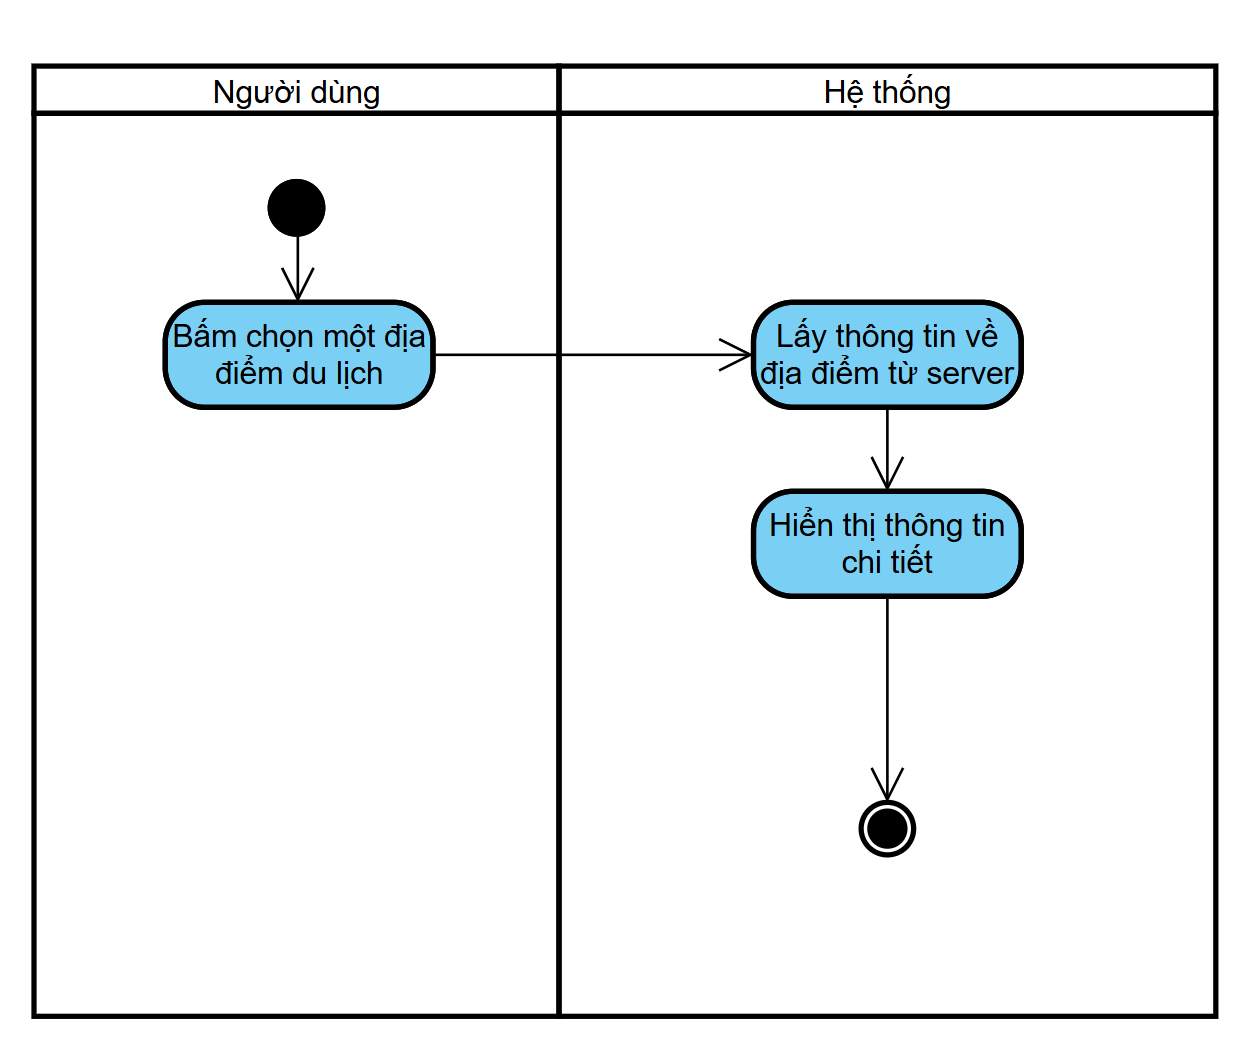
\includegraphics[width=0.5\linewidth]{figures/c3/3-3-8-ad.png} % Specified width
        &
        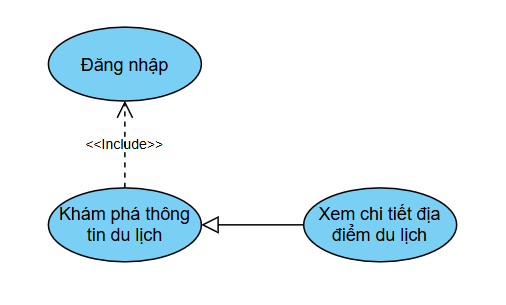
\includegraphics[width=0.45\linewidth]{figures/c3/3-3-8-rd.png} \\ % Specified width
        \hline
    \end{tabular}
\end{table}

\begin{figure}[H]
    \centering
    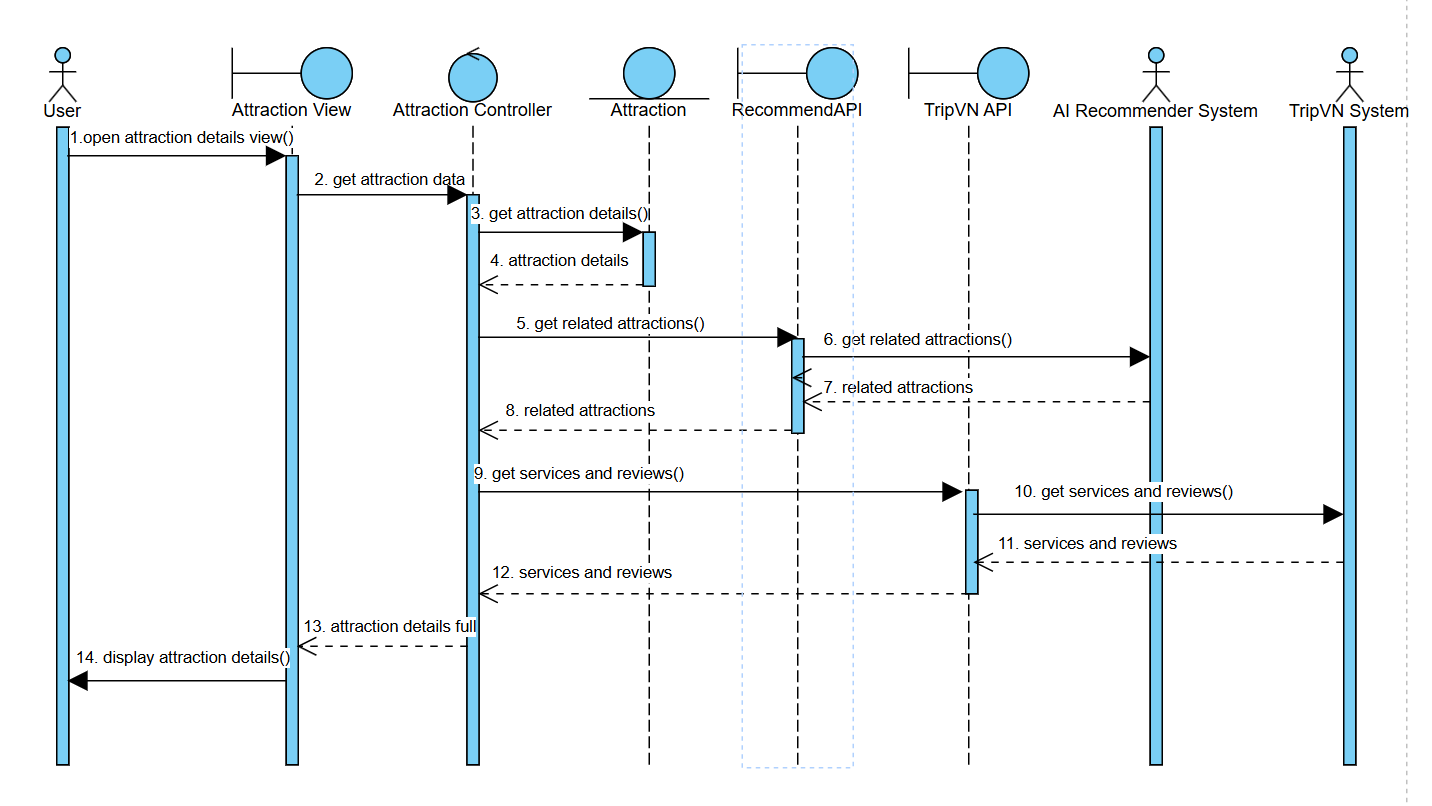
\includegraphics[width=1\textwidth]{figures/c3/3-3-8-sd.png} % Specified width
    \caption{Biểu đồ tuần tự ca sử dụng xem thông tin chi tiết địa điểm du lịch.}
    \label{fig:3-3-8-sequence-diagram}
\end{figure}
\nopagebreak
\subsection{Ca sử dụng gửi tin nhắn}
\vspace{0.5cm}


\noindent 
\begin{tabularx}{\linewidth}{| l | X |} 
\hline 
\textbf{Mô tả} & Người dùng có thể gửi tin nhắn trong nhóm hoặc gửi tin nhắn riêng cho bạn bè.  \\ 
\hline 
\textbf{Luồng cơ bản} & 1. Người dùng truy cập tab tin nhắn. \newline
                        2. Người dùng bấm vào một cuộc hội thoại muốn gửi tin nhắn. \newline
                        3. Hệ thống hiển thị thông tin của cuộc hội thoại và các tin nhắn trong cuộc hội thoại đó. \newline
                        4. Người dùng nhập tin nhắn muốn gửi. \newline
                        5. Người dùng bấm gửi. \newline
                        6. Hệ thống gửi tin nhắn và hiển thị tin nhắn vừa gửi lên cuộc hội thoại. \\
                        
\hline 
\textbf{Luồng thay thế} & Người dùng đính kèm địa điểm vào tin nhắn \newline
   1. Người dùng nhấn nút "+" cạnh ô input. \newline
   2. Hệ thống hiển thị giao diện tìm kiếm/chọn địa điểm. \newline
   3. Người dùng chọn một địa điểm. \newline
   4. Hệ thống thêm thông tin địa điểm đã chọn vào nội dung tin nhắn đang soạn thảo. \\

                       
\hline 
\textbf{Tiền điều kiện} &- Người dùng đang đăng nhập và phiên đăng nhập chưa kết thúc. \newline
                        - Người dùng đã có ít nhất một cuộc hội thoại. \\
\hline 
\textbf{Hậu điều kiện} & - Hệ thống lưu tin nhắn vào cơ sở dữ liệu và hiển thị tin nhắn trong cuộc hội thoại trong thời gian thực. \newline
                        - Hệ thống nhận diện địa điểm trong tin nhắn và highlight các địa điểm đó. \newline
                        - Hệ thống phân loại tin nhắn có cần thiết cho tổng hợp lịch trìn hay không. \newline
                        - Người dùng có thể nhấn vào địa điểm trong tin nhắn để xem chi tiết địa điểm. \newline
                        - Người dùng có thể react hoặc gỡ tin nhắn\\

\hline 
\textbf{Yêu cầu phi chức năng} & Hệ thống xử lý gửi tin nhắn dưới 1s  \\ 
\hline 
\end{tabularx}



\noindent 
\begin{tabular}{| c | c |}
    \hline
    \textbf{Biểu đồ hoạt động} & \textbf{Quan hệ} \\ 
    \hline
    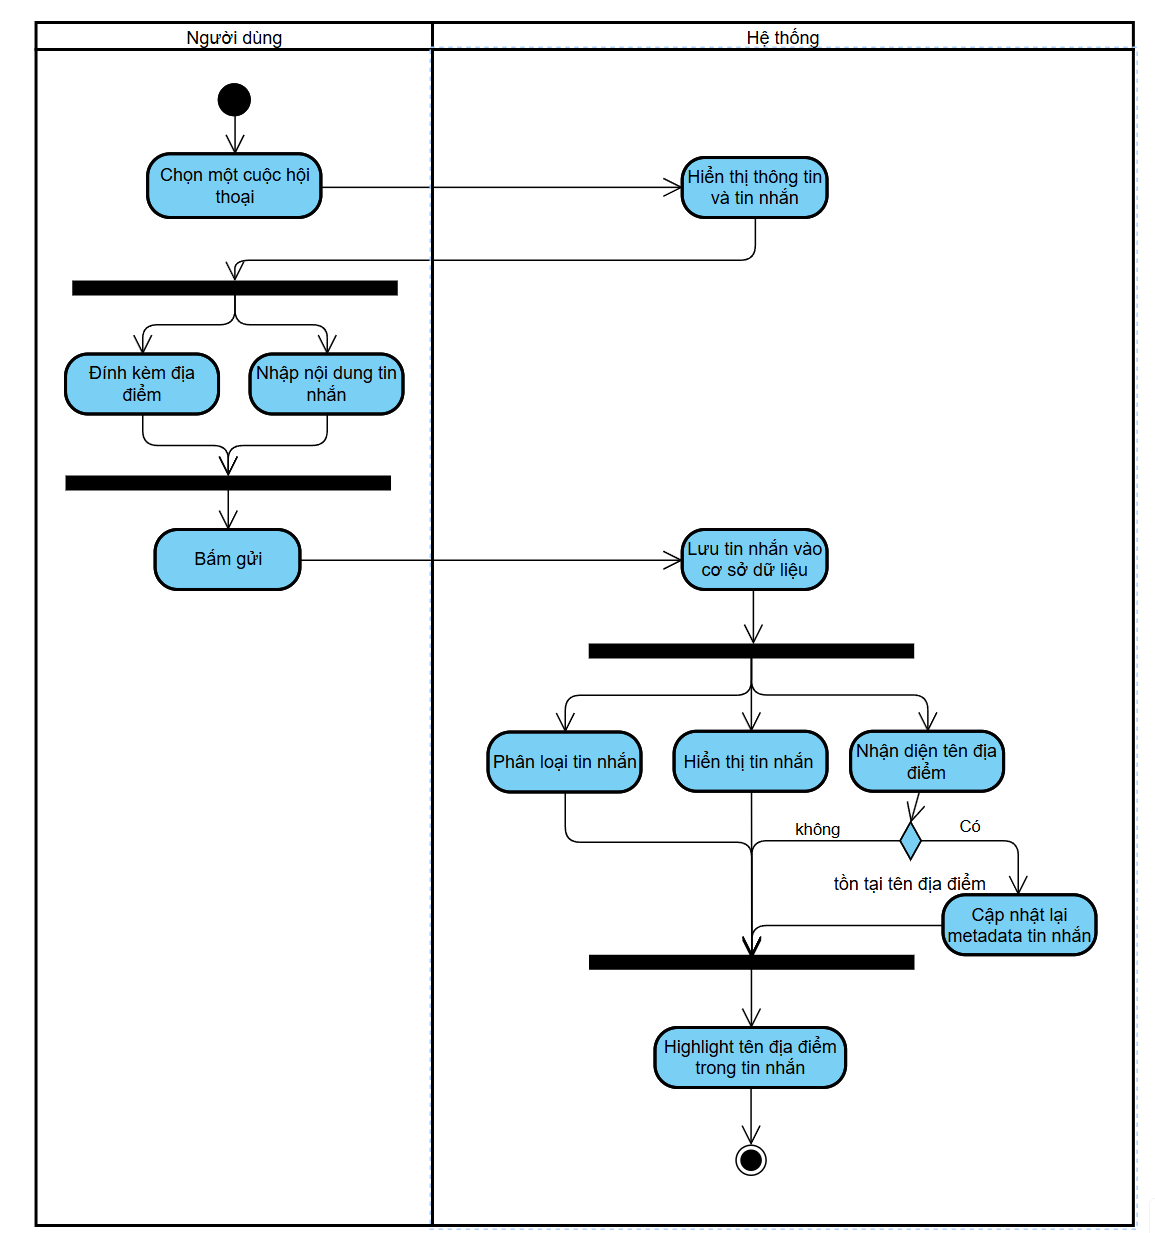
\includegraphics[width=0.5\linewidth]{figures/c3/3-3-9-ad.png} 
    & 
    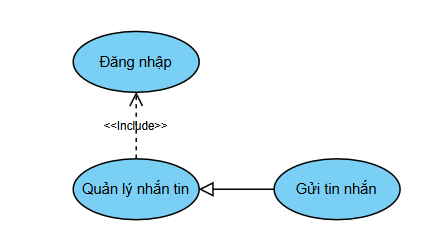
\includegraphics[width=0.45\linewidth]{figures/c3/3-3-9-rd.png} \\ 
    \hline
\end{tabular}


\vspace{0.8cm}

\begin{figure}[H]
    \centering  
    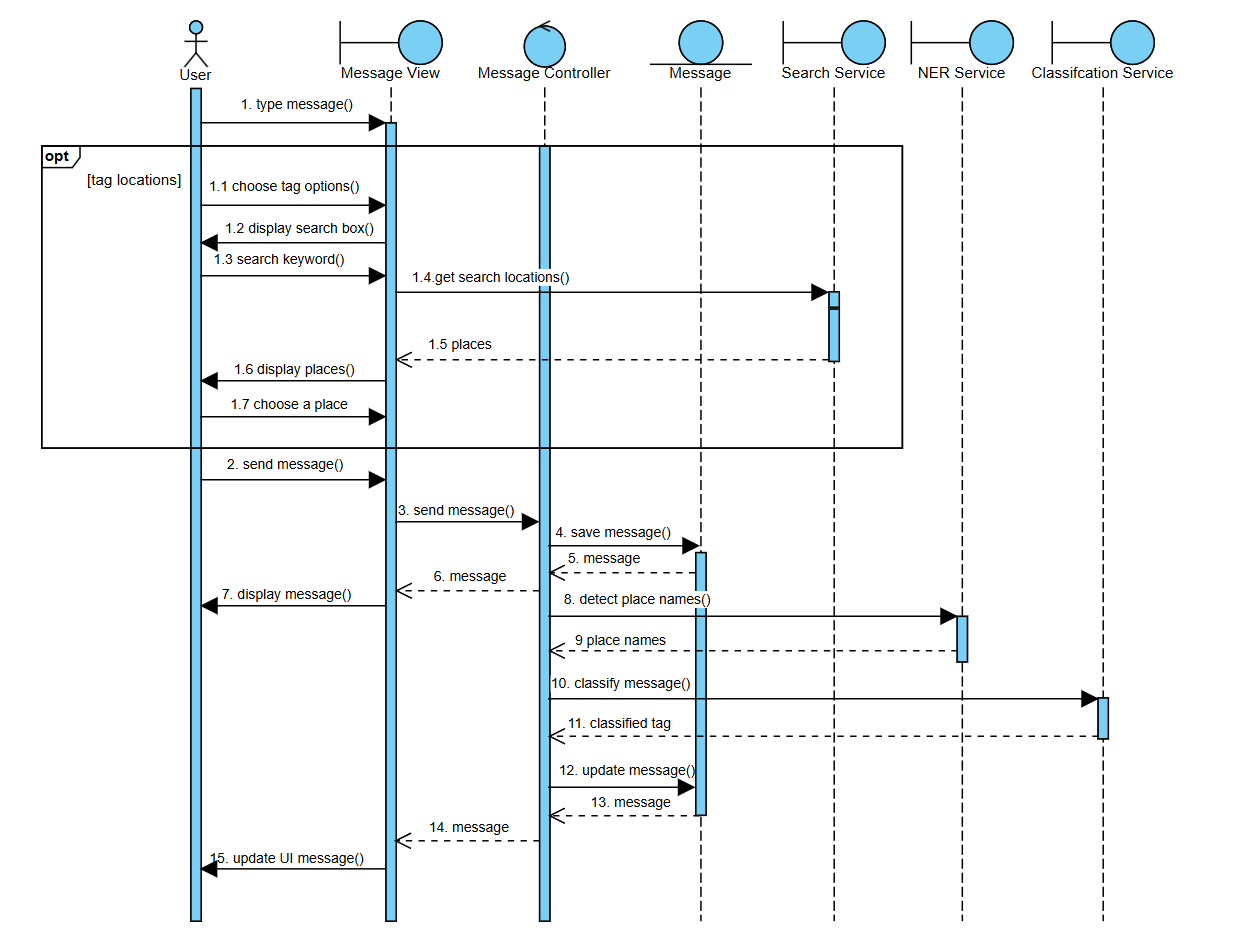
\includegraphics[width=1\textwidth]{figures/c3/3-3-9-sd.png}
    \caption{Biểu đồ tuần tự ca sử dụng gửi tin nhắn.}
    \label{fig:3-3-9-sequence-diagram}
\end{figure}
\nopagebreak
\subsection{Ca sử dụng tổng hợp lịch trình từ hội thoại}
\vspace{0.5cm}


\noindent 
\begin{tabularx}{\linewidth}{| l | X |} 
\hline 
\textbf{Mô tả} & Hệ thống sẽ tổng hợp lại lịch trình được đúc kết từ đoạn tin nhắn trong nhóm chat của người dùng.  \\ 
\hline 
\textbf{Luồng cơ bản} & 1. Người dùng bấm vào một cuộc hội thoại nhóm muốn tổng hợp. \newline
                        2. Hệ thống hiển thị thông cuộc hội thoại và các tin nhắn trong cuộc hội thoại đó. \newline
                        3. Người dùng chọn tùy chọn tổng hợp tin nhắn. \newline
                        4. Hệ thống lấy và hiển thị lịch trình tổng hợp của cuộc hội thoại (nếu có) . \newline
                        5. Người dùng bấm "Tổng hợp". \newline
                        6. Hệ thống sử dụng AI tổng hợp lịch trình trong cuộc hội thoại và hiển thị lịch trình tổng hợp. \\
                        
\hline 
\textbf{Luồng thay thế} & Hệ thống thông báo lỗi khi không có tin nhắn mới chưa được cập nhật. \\

                       
\hline 
\textbf{Tiền điều kiện} &- Người dùng đang đăng nhập và phiên đăng nhập chưa kết thúc. \newline
                        - Người dùng đã có ít nhất một cuộc hội thoại nhóm. \\
\hline 
\textbf{Hậu điều kiện} & - Hệ thống tổng hợp lịch trình sau đó lưu vào cơ sở dữ liệu và hiển thị cho người dùng. \newline
                        - Hệ thống đánh dấu các tin nhắn đã được tổng hợp. \newline
                        - Hệ thống gộp lịch trình với lịch trình đã tổng hợp trước đó.\\

\hline 
\textbf{Yêu cầu phi chức năng} & Hệ thống xử lý tổng hợp lịch trình dưới 10s  \\ 
\hline 
\end{tabularx}



\noindent 
\begin{tabular}{| c | c |}
    \hline
    \textbf{Biểu đồ hoạt động} & \textbf{Quan hệ} \\ 
    \hline
    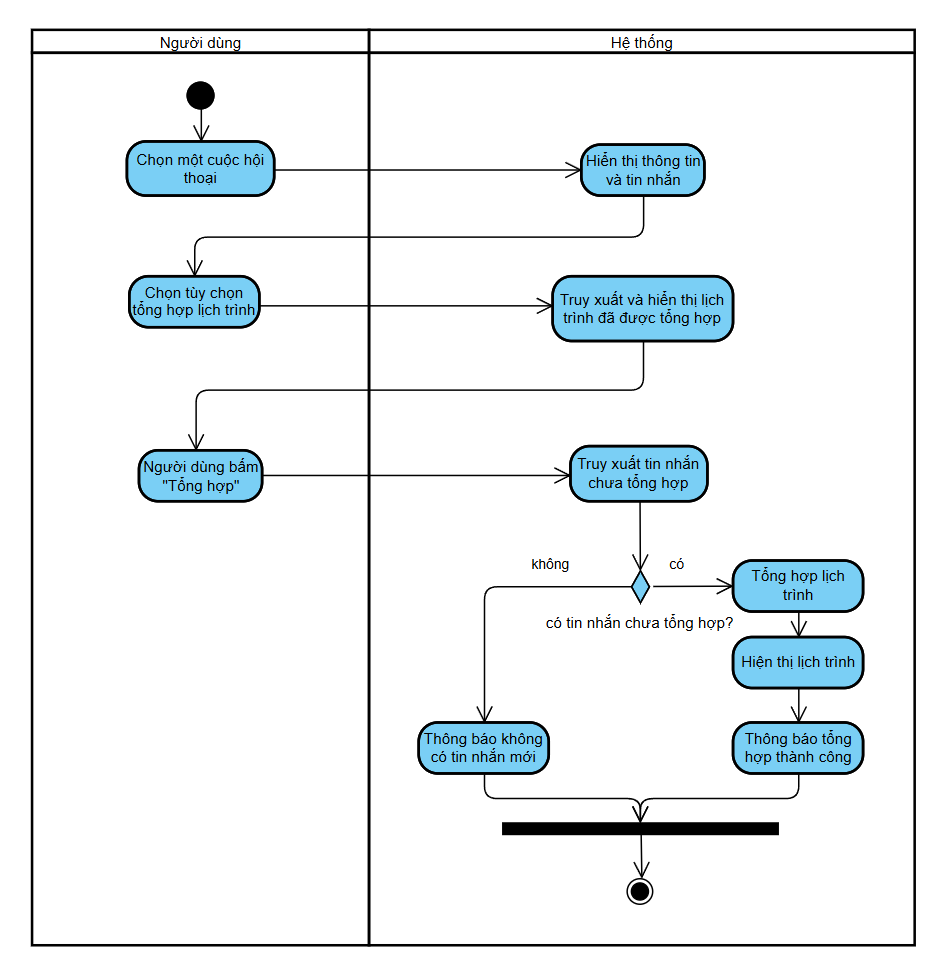
\includegraphics[width=0.5\linewidth]{figures/c3/3-3-10-ad.png} 
    & 
    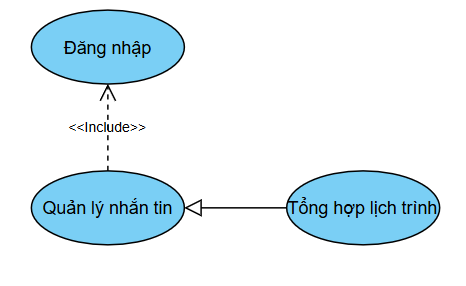
\includegraphics[width=0.45\linewidth]{figures/c3/3-3-10-rd.png} \\ 
    \hline
\end{tabular}


\vspace{0.8cm}

\begin{figure}[H]
    \centering  
    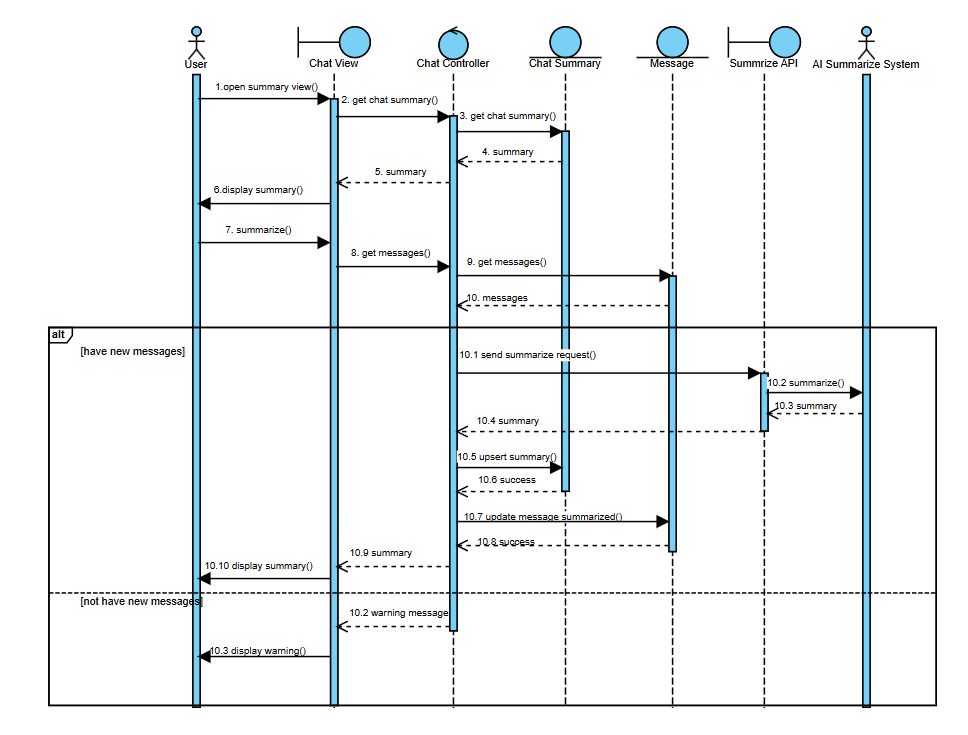
\includegraphics[width=1\textwidth]{figures/c3/3-3-10-sd.png}
    \caption{Biểu đồ tuần tự ca sử dụng tổng hợp lịch trình.}
    \label{fig:3-3-10-sequence-diagram}
\end{figure}
\nopagebreak
\subsection{Ca sử dụng tạo chuyến đi mặc định}
\noindent Ca sử dụng này mô tả cách người dùng tạo nhanh một chuyến đi mới chỉ với tên chuyến đi. Chuyến đi này mặc định sẽ ở chế độ riêng tư và người dùng có thể cập nhật chi tiết sau. Bảng~\ref{tab:uc_create_default_trip_spec} trình bày chi tiết đặc tả ca sử dụng, bao gồm luồng sự kiện chính, luồng thay thế, các điều kiện và yêu cầu liên quan. Các biểu đồ hoạt động, quan hệ (Bảng~\ref{tab:uc_create_default_trip_diagrams}) và tuần tự (Hình~\ref{fig:3-3-11-sequence-diagram}) minh họa rõ hơn về quy trình và tương tác hệ thống.
% \vspace{0.5cm} % Adjust spacing if needed

% Use longtable environment
% Need \usepackage{longtable} and \usepackage{calc} in preamble
\begin{longtable}{| p{4cm} | p{\dimexpr\linewidth-4cm-4\tabcolsep} |} % Adjust widths as needed
    \caption{Đặc tả ca sử dụng tạo chuyến đi mặc định} % Caption inside longtable
    \label{tab:uc_create_default_trip_spec} \\ % Label after caption

    \hline
    \textbf{Mô tả} & Người dùng có thể tạo chuyến đi để lên kế hoạch du lịch cho bản thân và bạn bè. \\
    \hline
    \endfirsthead % Header for the first page

    % No \endhead content needed

    % No \endfoot content needed

    \hline % Footer for the last page
    \endlastfoot

    % --- Table Content ---
    \textbf{Luồng cơ bản} & 1. Người dùng bấm vào tab chuyến đi. \newline
                           2. Người dùng bấm vào dấu ``+'' góc phải trên. \newline
                           3. Hệ thống hiển thị hộp thoại yêu cầu người dùng nhập tên cho chuyến đi. \newline
                           4. Người dùng nhập tên chuyến đi. \newline
                           5. Người dùng bấm ``Tạo". \newline
                           6. Hệ thống tạo một chuyến đi mới với tên đã đặt. \\
    \hline
    \textbf{Luồng thay thế} & Hệ thống thông báo lỗi khi tên chuyến đi dài hơn 80 kí tự. \\
    \hline
    \textbf{Tiền điều kiện} & - Người dùng đang đăng nhập và phiên đăng nhập chưa kết thúc. \\
    \hline
    \textbf{Hậu điều kiện} & - Hệ thống thêm chuyến đi với trạng thái là riêng tư của người dùng vào cơ sở dữ liệu. \\
    \hline
    \textbf{Yêu cầu phi chức năng} & Hệ thống tạo chuyến đi dưới 2s. \\
    % --- End Table Content ---

\end{longtable}


\begin{table}[H] % Wrap the diagrams table
    \centering
    \caption{Biểu đồ hoạt động và quan hệ ca sử dụng tạo chuyến đi mặc định} % Add caption
    \label{tab:uc_create_default_trip_diagrams} % Add label
    \begin{tabular}{| c | c |}
        \hline
        \textbf{Biểu đồ hoạt động} & \textbf{Quan hệ} \\
        \hline
        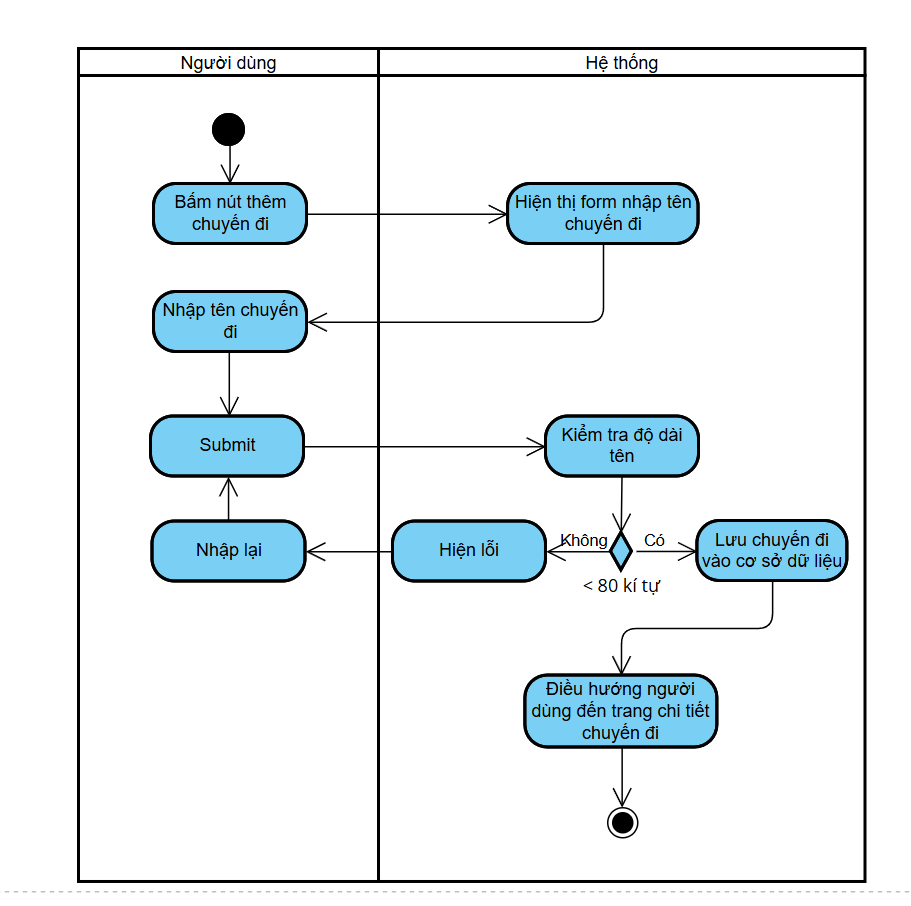
\includegraphics[width=0.5\linewidth]{figures/c3/3-3-11-ad.png} % Specified width
        &
        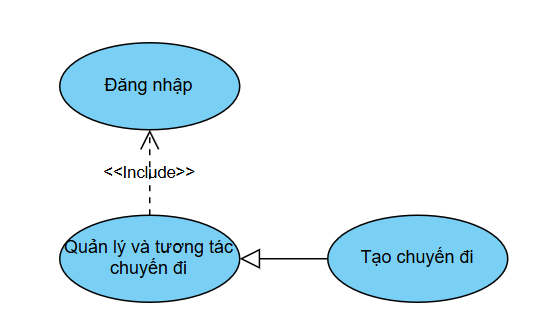
\includegraphics[width=0.45\linewidth]{figures/c3/3-3-11-rd.png} \\ % Specified width
        \hline
    \end{tabular}
\end{table}

\begin{figure}[H]
    \centering
    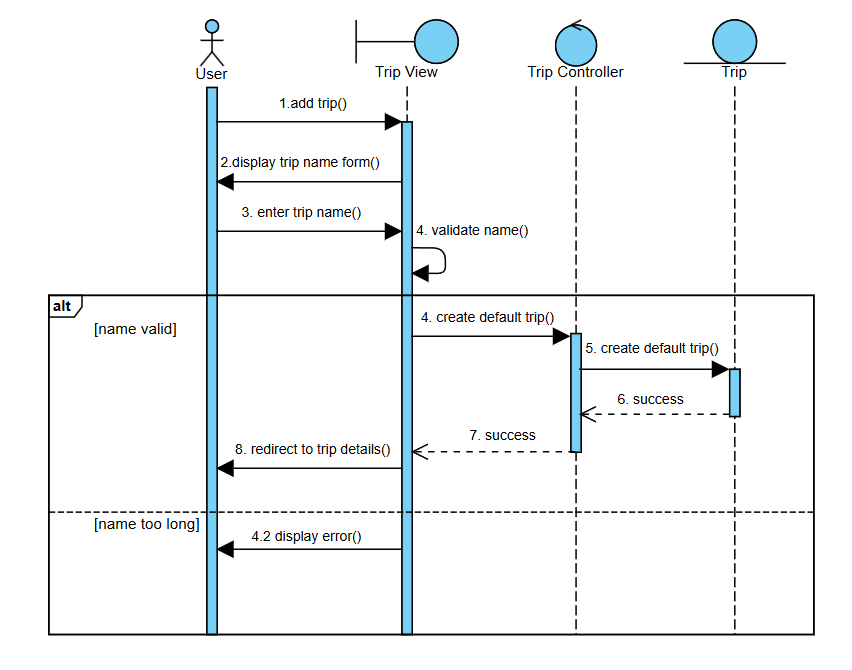
\includegraphics[width=0.95\textwidth]{figures/c3/3-3-11-sd.png} % Specified width
    \caption{Biểu đồ tuần tự ca sử dụng tạo chuyến đi mặc định.}
    \label{fig:3-3-11-sequence-diagram}
\end{figure}
\nopagebreak
\subsection{Ca sử dụng thêm mục lưu trữ vào chuyến đi}
\noindent Ca sử dụng này mô tả cách người dùng lưu các địa điểm, sự kiện, hoặc nhà hàng vào một chuyến đi cụ thể để tham khảo khi lên lịch trình. Người dùng có thể tìm kiếm và chọn các mục muốn lưu. Bảng~\ref{tab:uc_add_saved_item_spec} trình bày chi tiết đặc tả ca sử dụng, bao gồm luồng sự kiện chính, luồng thay thế, các điều kiện và yêu cầu liên quan. Các biểu đồ hoạt động, quan hệ (Bảng~\ref{tab:uc_add_saved_item_diagrams}) và tuần tự (Hình~\ref{fig:3-3-12-sequence-diagram}) minh họa rõ hơn về quy trình và tương tác hệ thống.
% \vspace{0.5cm} % Adjust spacing if needed

% Use longtable environment
% Need \usepackage{longtable} and \usepackage{calc} in preamble
\begin{longtable}{| p{4cm} | p{\dimexpr\linewidth-4cm-4\tabcolsep} |} % Adjust widths as needed
    \caption{Đặc tả ca sử dụng thêm mục lưu trữ vào chuyến đi} % Caption inside longtable (no period)
    \label{tab:uc_add_saved_item_spec} \\ % Label after caption

    \hline
    \textbf{Mô tả} & Người dùng có thể lưu các địa điểm, sự kiện, nhà hàng vào chuyến đi để lên lịch trình dựa trên nó. \\
    \hline
    \endfirsthead % Header for the first page

    % No \endhead content needed

    % No \endfoot content needed

    \hline % Footer for the last page
    \endlastfoot

    % --- Table Content ---
    \textbf{Luồng cơ bản} & 1. Người dùng chọn một chuyến đi muốn thêm mục lưu. \newline
                           2. Hệ thống lấy dữ liệu chi tiết của chuyến đi và hiển thị. \newline
                           3. Người dùng bấm ``Thêm mục lưu". \newline
                           4. Hệ thống điều hướng sang trang thêm mục lưu và hiển thị thanh tìm kiếm. \newline
                           5. Người dùng nhập tên địa điểm, sự kiện hoặc nhà hàng muốn thêm vào chuyến đi. \newline
                           6. Hệ thống tìm kiếm và hiển thị danh sách các mục lưu phù hợp với từ khóa tìm kiếm. \newline
                           7. Người dùng chọn mục muốn lưu trong danh sách. \newline
                           8. Hệ thống thông báo đã thêm thành công. \\
    \hline
    \textbf{Luồng thay thế} & Người dùng bấm vào mục đã lưu sẽ bỏ lưu mục đấy. \\
    \hline
    \textbf{Tiền điều kiện} & - Người dùng đang đăng nhập và phiên đăng nhập chưa kết thúc.\newline
                           - Người dùng đã tạo hoặc tham gia ít nhất một chuyến đi. \newline
                           - Trạng thái chuyến đi khác ``Đã hoàn thành'' và ``Hủy". \\
    \hline
    \textbf{Hậu điều kiện} & - Hệ thống thêm mục lưu của chuyến đi vào cơ sở dữ liệu.\newline
                           - Người dùng có thể xem lại mục lưu đã thêm vào chuyến đi. \\
    \hline
    \textbf{Yêu cầu phi chức năng} & Hệ thống thêm mục lưu dưới 1s. \\
    % --- End Table Content ---

\end{longtable}


\begin{table}[H] % Wrap the diagrams table
    \centering
    \caption{Biểu đồ hoạt động ca sử dụng thêm mục lưu trữ vào chuyến đi} % Add caption (no period)
    \label{tab:uc_add_saved_item_diagrams} % Add label
    \begin{tabular}{| c | c |}
        \hline
        \textbf{Biểu đồ hoạt động} & \textbf{Quan hệ} \\
        \hline
        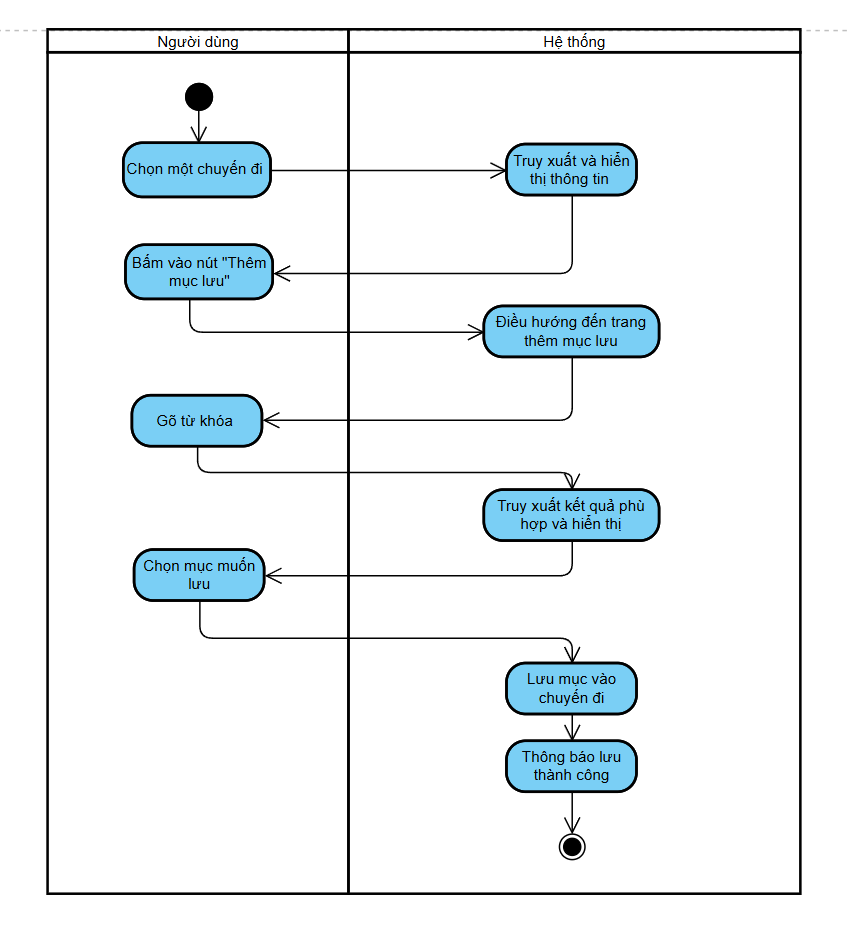
\includegraphics[width=0.5\linewidth]{figures/c3/3-3-12-ad.png} % Specified width
        &
        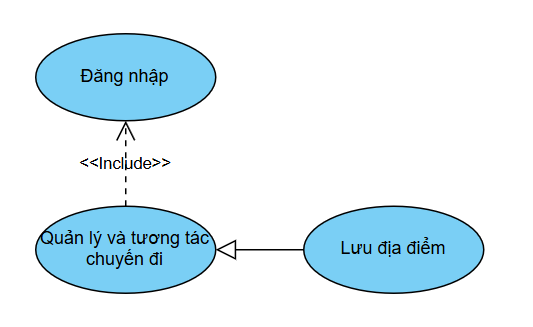
\includegraphics[width=0.45\linewidth]{figures/c3/3-3-12-rd.png} \\ % Specified width
        \hline
    \end{tabular}
\end{table}

\begin{figure}[H]
    \centering
    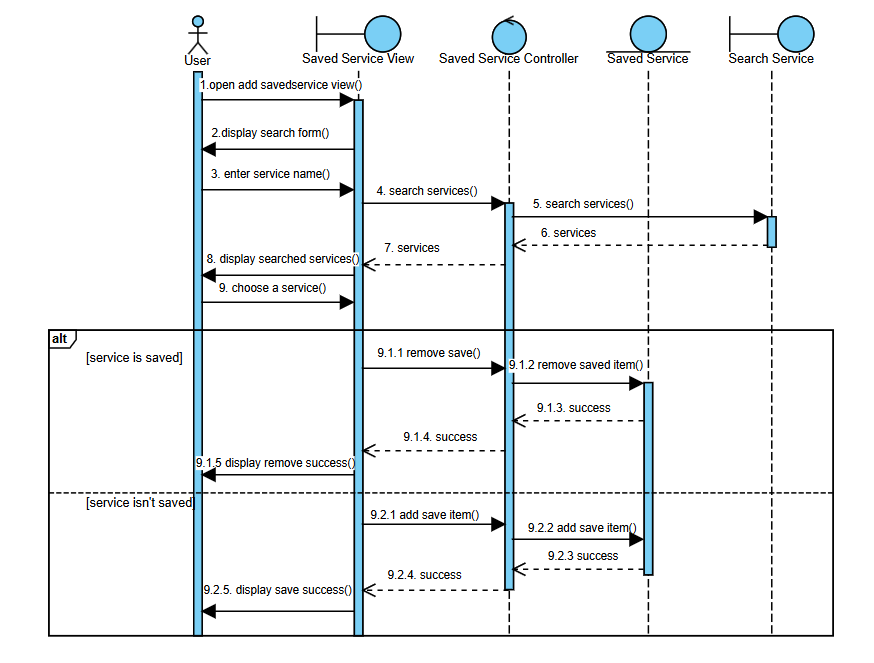
\includegraphics[width=0.92\textwidth]{figures/c3/3-3-12-sd.png} % Specified width
    \caption{Biểu đồ tuần tự ca sử dụng thêm mục lưu vào chuyến đi.} % (no period)
    \label{fig:3-3-12-sequence-diagram}
\end{figure}
\nopagebreak
\subsection{Ca sử dụng tạo lịch trình cho chuyến đi}
\noindent Ca sử dụng này mô tả cách người dùng tạo một mục lịch trình cụ thể cho một ngày trong chuyến đi của họ. Người dùng có thể chọn địa điểm từ danh sách đã lưu hoặc chọn trực tiếp trên bản đồ, sau đó cung cấp thông tin chi tiết như thời gian và ghi chú. Bảng~\ref{tab:uc_create_itinerary_item_spec} trình bày chi tiết đặc tả ca sử dụng, bao gồm luồng sự kiện chính, luồng thay thế, các điều kiện và yêu cầu liên quan. Các biểu đồ hoạt động, quan hệ (Bảng~\ref{tab:uc_create_itinerary_item_diagrams}) và tuần tự (Hình~\ref{fig:3-3-13-sequence-diagram}) minh họa rõ hơn về quy trình và tương tác hệ thống.
% \vspace{0.5cm} % Adjust spacing if needed

% Use longtable environment
% Need \usepackage{longtable} and \usepackage{calc} in preamble
\begin{longtable}{| p{4cm} | p{\dimexpr\linewidth-4cm-4\tabcolsep} |} % Adjust widths as needed
    \caption{Đặc tả ca sử dụng tạo lịch trình cho chuyến đi} % Caption inside longtable (no period)
    \label{tab:uc_create_itinerary_item_spec} \\ % Label after caption

    \hline
    \textbf{Mô tả} & Người dùng có thể tạo một lịch trình cụ thể cho chuyến đi của mình. \\
    \hline
    \endfirsthead % Header for the first page

    % No \endhead content needed

    % No \endfoot content needed

    \hline % Footer for the last page
    \endlastfoot

    % --- Table Content ---
    \textbf{Luồng cơ bản} & 1. Người dùng chọn một chuyến đi. \newline
                           2. Hệ thống lấy dữ liệu chi tiết và hiển thị. \newline
                           3. Người dùng bấm ``Thêm lịch trình". \newline
                           4. Hệ thống hiển thị 2 lựa chọn tạo lịch trình. \newline
                           5. Người dùng chọn tùy chọn ``chọn từ mục lưu". \newline
                           6. Hệ thống truy xuất và hiển thị các mục lưu của chuyến đi cho người dùng chọn. \newline
                           7. Người dùng chọn mục thêm vào lịch trình. \newline
                           8. Hệ thống hiển thị form điền thông tin lịch trình. \newline
                           9. Người dùng điền thông tin lịch trình như thời gian bắt đầu, ghi chú,v.v. \newline
                           10. Người dùng bấm ``Lưu lịch trình". \newline
                           11. Hệ thống lưu lịch trình vào cơ sở dữ liệu và thông báo thành công. \\
    \hline
    \textbf{Luồng thay thế} & \textbf{Chọn trên bản đồ:} \newline
                               1. Người dùng chọn tùy chọn ``chọn trên bản đồ". \newline
                               2. Hệ thống hiển thị bản đồ. \newline
                               3. Người dùng chọn 1 vị trí trên bản đồ. \newline
                               4. Tiếp tục từ bước 8 của Luồng cơ bản. \\
    \hline
    \textbf{Tiền điều kiện} & - Người dùng đang đăng nhập và phiên đăng nhập chưa kết thúc.\newline
                           - Người dùng đã tạo hoặc tham gia ít nhất một chuyến đi. \newline
                           - Trạng thái chuyến đi khác ``Đã hoàn thành'' và ``Hủy". \\
    \hline
    \textbf{Hậu điều kiện} & - Hệ thống lưu lịch trình vào cơ sở dữ liệu.\newline
                           - Người dùng có thể chỉnh sửa lịch trình đã tạo. \newline
                           - Người dùng có thể xem bản đồ trực quan lịch trình đã tạo. \\
    \hline
    \textbf{Yêu cầu phi chức năng} & Hệ thống thêm mục lưu dưới 2s \\
    % --- End Table Content ---

\end{longtable}
\vspace{0.8cm}

\begin{table}[H] % Wrap the diagrams table
    \centering
    \caption{Biểu đồ hoạt động và quan hệ ca sử dụng tạo lịch trình cho chuyến đi} % Add caption (no period)
    \label{tab:uc_create_itinerary_item_diagrams} % Add label
    \begin{tabular}{| c | c |}
        \hline
        \textbf{Biểu đồ hoạt động} & \textbf{Quan hệ} \\
        \hline
        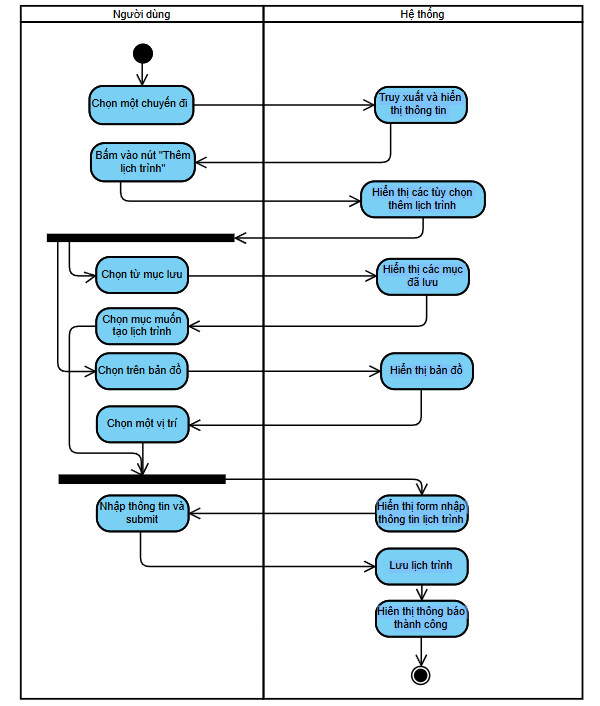
\includegraphics[width=0.5\linewidth]{figures/c3/3-3-13-ad.png} % Specified width
        &
        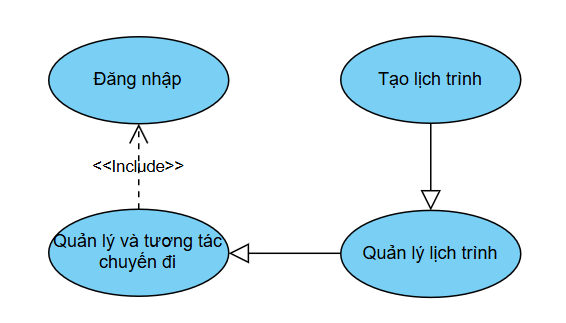
\includegraphics[width=0.45\linewidth]{figures/c3/3-3-13-rd.png} \\ % Specified width
        \hline
    \end{tabular}
\end{table}

\begin{figure}[H]
    \centering
    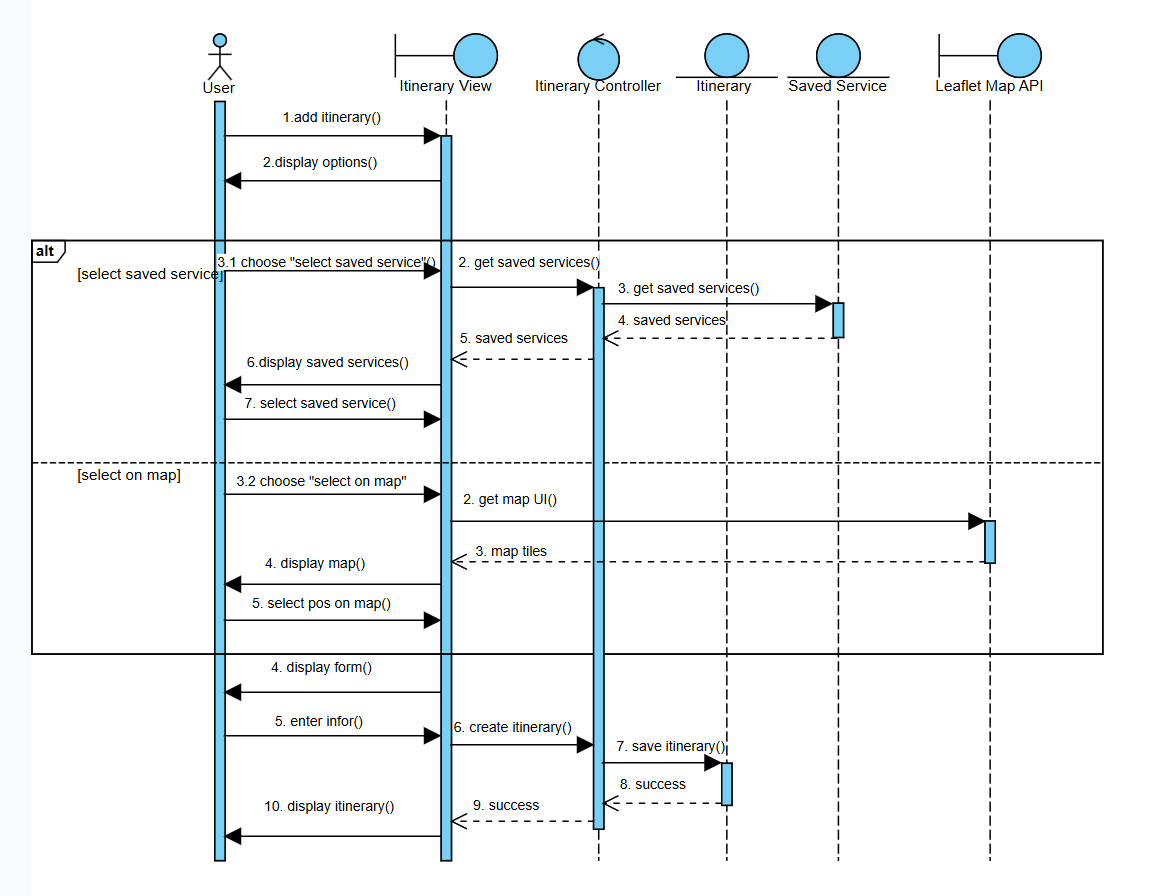
\includegraphics[width=1\textwidth]{figures/c3/3-3-13-sd.png} % Specified width
    \caption{Biểu đồ tuần tự ca sử dụng tạo lịch trình cho chuyến đi.} % (no period)
    \label{fig:3-3-13-sequence-diagram}
\end{figure}
\nopagebreak
% \subsection{Ca sử dụng mời bạn bè tham gia chuyến đi}
\noindent Ca sử dụng này mô tả cách người dùng mời bạn bè của họ tham gia vào một chuyến đi công khai mà họ đã tạo hoặc đang tham gia. Hệ thống sẽ gửi thông báo mời đến những người được chọn. Bảng~\ref{tab:uc_invite_friend_spec} trình bày chi tiết đặc tả ca sử dụng, bao gồm luồng sự kiện chính, luồng thay thế, các điều kiện và yêu cầu liên quan. Các biểu đồ hoạt động, quan hệ (Bảng~\ref{tab:uc_invite_friend_diagrams}) và tuần tự (Hình~\ref{fig:3-3-14-sequence-diagram}) minh họa rõ hơn về quy trình và tương tác hệ thống khi mời bạn bè.
% \vspace{0.5cm} % Adjust spacing if needed

% Use longtable environment
% Need \usepackage{longtable} and \usepackage{calc} in preamble
\begin{longtable}{| p{4cm} | p{\dimexpr\linewidth-4cm-4\tabcolsep} |} % Adjust widths as needed
    \caption{Đặc tả ca sử dụng mời bạn bè tham gia chuyến đi} % Caption inside longtable (no period)
    \label{tab:uc_invite_friend_spec} \\ % Label after caption

    \hline
    \textbf{Mô tả} & Người dùng có thể mời bạn bè tham gia chuyến đi của mình hoặc mình tham gia. \\
    \hline
    \endfirsthead % Header for the first page

    % No \endhead content needed

    % No \endfoot content needed

    \hline % Footer for the last page
    \endlastfoot

    % --- Table Content ---
    \textbf{Luồng cơ bản} & 1. Người dùng chọn một chuyến đi muốn mời bạn bè. \newline
                           2. Hệ thống lấy dữ liệu chi tiết của chuyến đi và hiển thị. \newline
                           3. Người dùng bấm ``Mời thành viên". \newline
                           4. Hệ thống điều hướng sang trang thêm thành viên và hiển thị thanh tìm kiếm. \newline
                           5. Người dùng nhập tên thành viên muốn mời. \newline
                           6. Hệ thống tìm kiếm và hiển thị danh sách các tài khoản phù hợp với từ khóa tìm kiếm. \newline
                           7. Người dùng chọn các tài khoản muốn mời. \newline
                           8. Hệ thống gửi thông báo mời vào chuyến đi và thông báo đã mời thành công. \\
    \hline
    \textbf{Luồng thay thế} & Người dùng được mời đã tham gia hoặc đã từ chối sẽ không được gửi thông báo tiếp. \\
    \hline
    \textbf{Tiền điều kiện} & - Người dùng đang đăng nhập và phiên đăng nhập chưa kết thúc.\newline
                           - Người dùng đã tạo hoặc tham gia ít nhất một chuyến đi. \newline
                           - Chuyến đi phải là chuyến đi công khai.\newline
                           - Trạng thái chuyến đi khác ``Đã hoàn thành'' và ``Hủy". \\
    \hline
    \textbf{Hậu điều kiện} & - Hệ thống gửi thông báo mời vào chuyến đi cho các tài khoản được chọn. \\
    \hline
    \textbf{Yêu cầu phi chức năng} & Hệ thống gửi lời mời bạn bè dưới 1s với 1 tài khoản. \\
    % --- End Table Content ---

\end{longtable}
\vspace{0.8cm}

\begin{table}[H] % Wrap the diagrams table
    \centering
    \caption{Biểu đồ hoạt động ca sử dụng mời bạn bè tham gia chuyến đi} % Add caption (no period)
    \label{tab:uc_invite_friend_diagrams} % Add label
    \begin{tabular}{| c | c |}
        \hline
        \textbf{Biểu đồ hoạt động} & \textbf{Quan hệ} \\
        \hline
        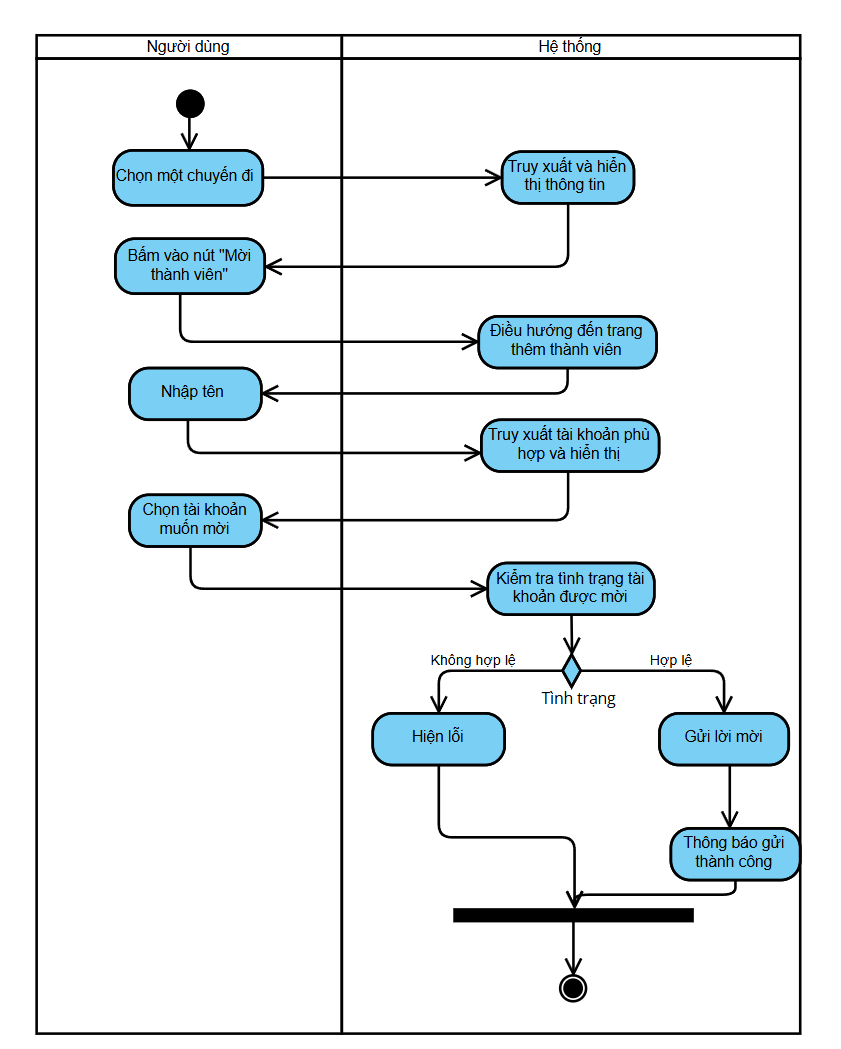
\includegraphics[width=0.5\linewidth]{figures/c3/3-3-14-ad.png} % Specified width
        &
        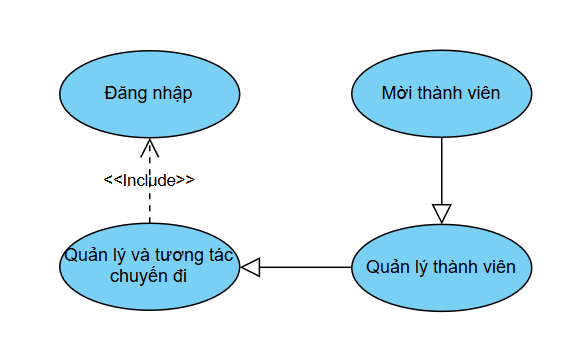
\includegraphics[width=0.45\linewidth]{figures/c3/3-3-14-rd.png} \\ % Specified width
        \hline
    \end{tabular}
\end{table}

\begin{figure}[H]
    \centering
    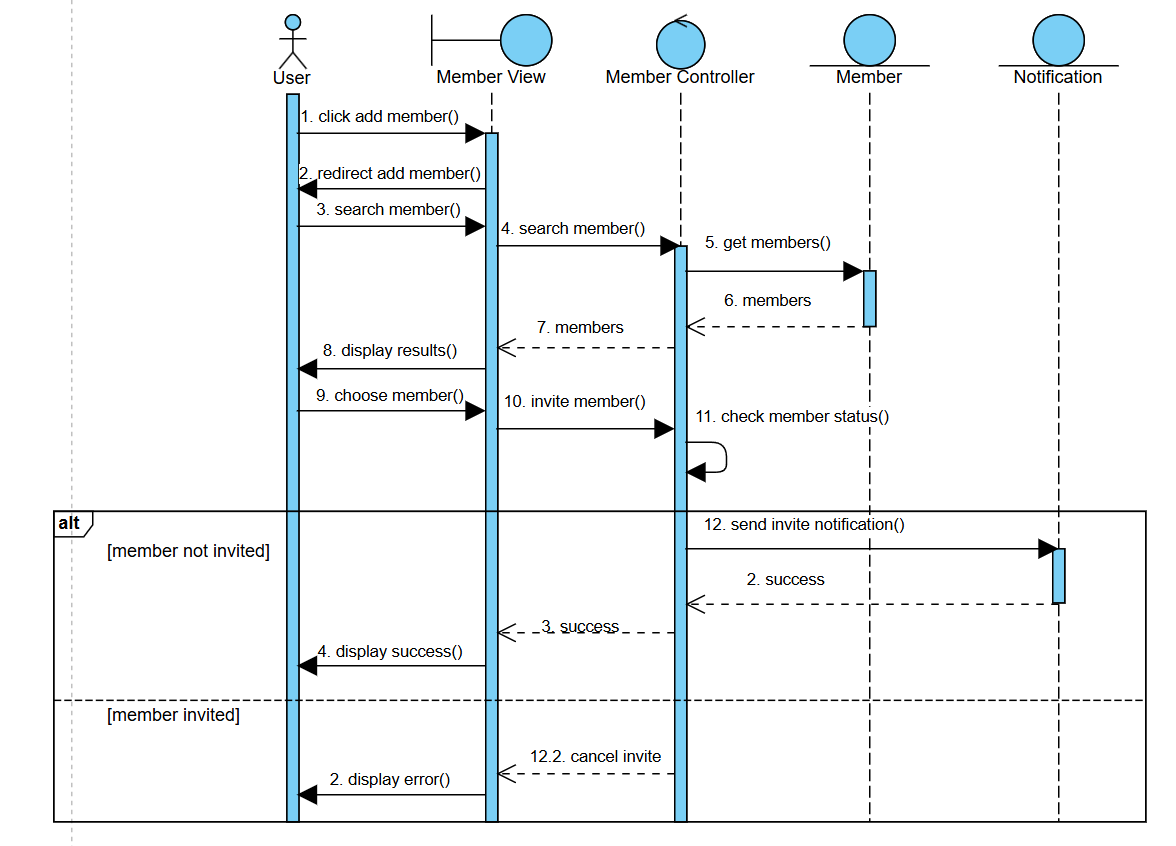
\includegraphics[width=0.85\textwidth]{figures/c3/3-3-14-sd.png} % Specified width
    \caption{Biểu đồ tuần tự ca sử dụng mời bạn bè tham gia chuyến đi.} % (no period)
    \label{fig:3-3-14-sequence-diagram}
\end{figure}
% \nopagebreak
% \subsection{Ca sử dụng công khai chuyến đi}
\vspace{0.5cm}


\noindent 
\begin{tabularx}{\linewidth}{| l | X |} 
\hline 
\textbf{Mô tả} & Người dùng công khai chuyến đi để mọi người tham gia. \\
\hline 
\textbf{Luồng cơ bản} & 1. Người dùng chọn một chuyến đi muốn công khai. \newline
                        2. Hệ thống lây dữ liệu chi tiết của chuyến đi và hiển thị. \newline
                        3. Người dùng bấm "Công khai". \newline
                        4. Hệ thống kiểm tra thông tin chuyến đi. \newline
                        5. Hệ thống chuyển đổi chuyến đi sang công khai và thông báo đến các tài khoản khác. \\
             
               
\hline 
\textbf{Luồng thay thế} & Chuyến đi không đủ thông tin hệ thống sẽ thông báo lỗi chưa đủ thông tin. \\
       
\hline 
\textbf{Tiền điều kiện} & - Người dùng đang đăng nhập và phiên đăng nhập chưa kết thúc.\newline
                        - Người dùng đã tạo ít nhất một chuyến đi. \newline
                        - Chuyến đi phải là chuyến di riêng tư.\\


\hline 
\textbf{Hậu điều kiện} & - Hệ thống cập nhật quyền riêng tư của chuyến đi sang công khai. \newline
- Hệ thống hiển thị chuyến đi dưới dạng bài viết trên trang chủ để mọi người tham gia. \newline
- Hệ thống gửi thông báo đến các tài khoản khác về chuyến đi công khai. \\
                        

\hline 
\textbf{Yêu cầu phi chức năng} & Hệ thống công khai chuyến đi dưới 2s \\
\hline 
\end{tabularx}

\noindent 
\begin{tabular}{| c | c |}
    \hline
    \textbf{Biểu đồ hoạt động} & \textbf{Quan hệ} \\ 
    \hline
    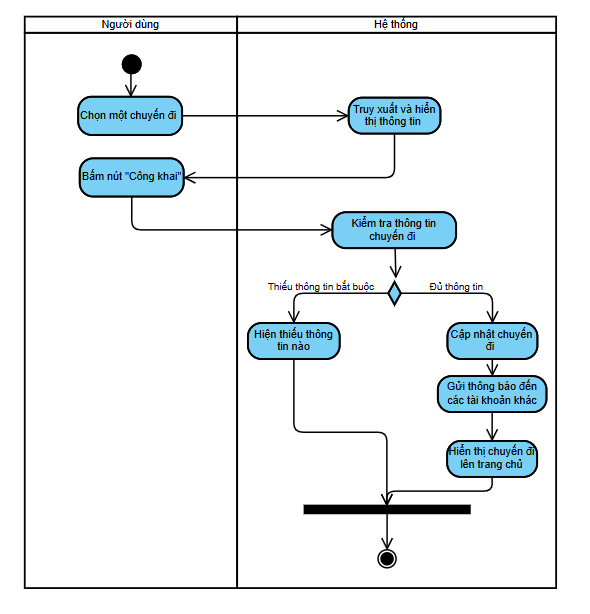
\includegraphics[width=0.5\linewidth]{figures/c3/3-3-15-ad.png} 
    & 
    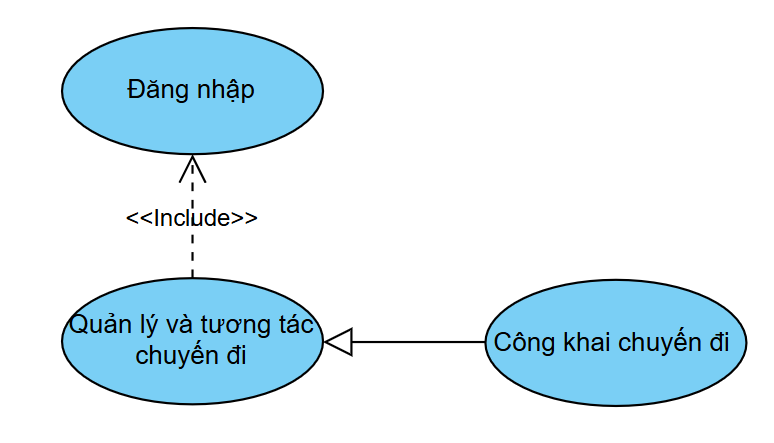
\includegraphics[width=0.45\linewidth]{figures/c3/3-3-15-rd.png} \\ 
    \hline
\end{tabular}

\vspace{0.8cm}

\begin{figure}[H]
    \centering  
    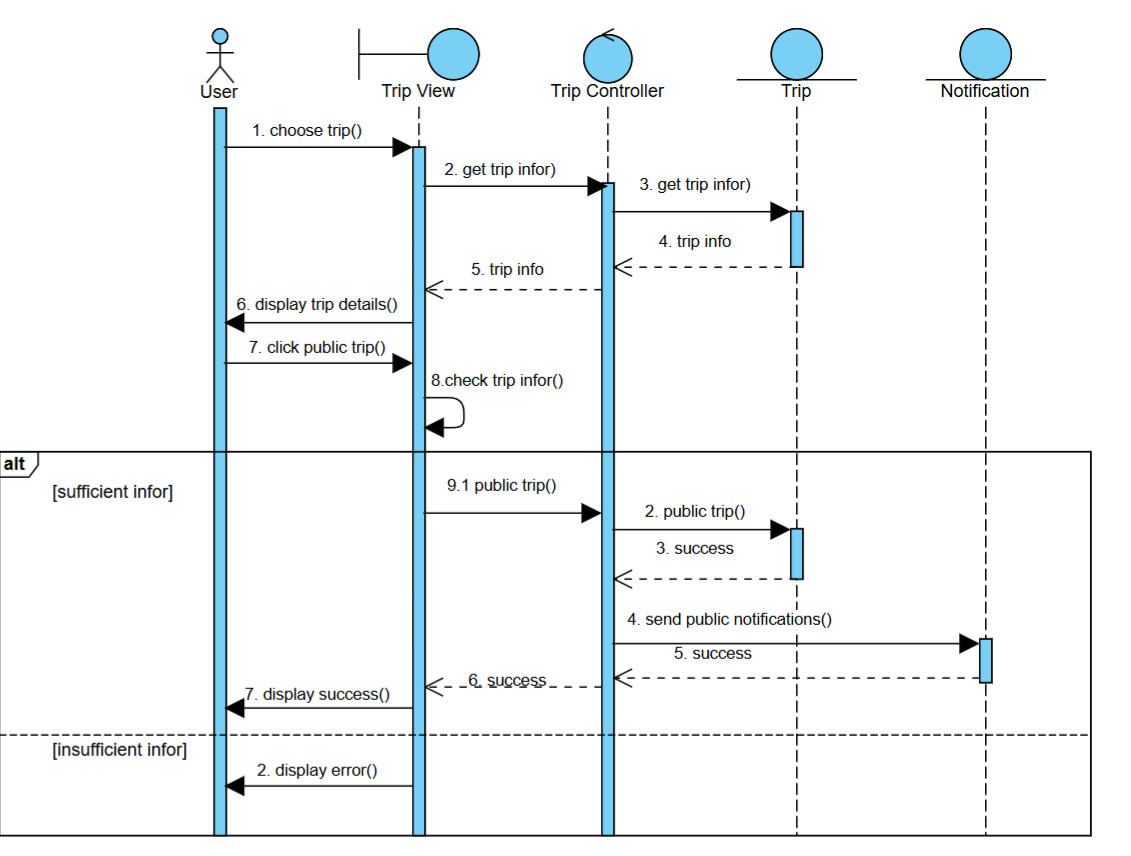
\includegraphics[width=1\textwidth]{figures/c3/3-3-15-sd.png}
    \caption{Biểu đồ tuần tự ca sử dụng công khai chuyến đi.}
    \label{fig:3-3-15-sequence-diagram}
\end{figure}
% \nopagebreak
\subsection{Ca sử dụng chia sẻ vị trí}
\noindent Ca sử dụng này mô tả cách người dùng chia sẻ vị trí thời gian thực của họ với các thành viên khác trong cùng một chuyến đi đang diễn ra. Tính năng này giúp các thành viên dễ dàng tìm thấy nhau hoặc theo dõi tiến trình di chuyển. Bảng~\ref{tab:uc_share_location_spec} trình bày chi tiết đặc tả ca sử dụng, bao gồm luồng sự kiện chính, luồng thay thế, các điều kiện và yêu cầu liên quan. Các biểu đồ hoạt động, quan hệ (Bảng~\ref{tab:uc_share_location_diagrams}) và tuần tự (Hình~\ref{fig:3-3-16-sequence-diagram}) minh họa rõ hơn về quy trình và tương tác hệ thống.
% \vspace{0.5cm} % Adjust spacing if needed

% Use longtable environment
% Need \usepackage{longtable} and \usepackage{calc} in preamble
\begin{longtable}{| p{4cm} | p{\dimexpr\linewidth-4cm-4\tabcolsep} |} % Adjust widths as needed
    \caption{Đặc tả ca sử dụng chia sẻ vị trí} % Caption inside longtable (no period)
    \label{tab:uc_share_location_spec} \\ % Label after caption

    \hline
    \textbf{Mô tả} & Người dùng trong cùng chuyến đi có thể chia sẻ vị trí khi chuyến đi đang diễn ra. \\
    \hline
    \endfirsthead % Header for the first page

    % No \endhead content needed

    % No \endfoot content needed

    \hline % Footer for the last page
    \endlastfoot

    % --- Table Content ---
    \textbf{Luồng cơ bản} & 1. Người dùng chọn một chuyến đi đang diễn ra. \newline
                           2. Hệ thống lấy dữ liệu chi tiết của chuyến đi và hiển thị. \newline
                           3. Người dùng bấm ``Chia sẻ vị trí". \newline
                           4. Hệ thống điều hướng người dùng ra trang hiển thị bản đồ. \newline
                           5. Hệ thống yêu cầu quyền truy cập vị trí liên tục. \newline
                           6. Người dùng cấp quyền. \newline
                           7. Hệ thống cập nhật liên tục trong thời gian thực vị trí của bản thân người dùng và các người dùng khác tham gia chia sẻ vị trí trong chuyến đi. \\
    \hline
    \textbf{Luồng thay thế} & Nếu người dùng không cấp quyền truy cập vị trí, hệ thống sẽ không thể chia sẻ vị trí của họ và chỉ hiển thị vị trí của các thành viên khác (nếu có). \\
    \hline
    \textbf{Tiền điều kiện} & - Người dùng đang đăng nhập và phiên đăng nhập chưa kết thúc.\newline
                           - Người dùng đã tạo hoặc tham gia ít nhất một chuyến đi. \newline
                           - Chuyến đi đang trong trạng thái ``Đang diễn ra". \\
    \hline
    \textbf{Hậu điều kiện} & - Hệ thống cập nhật vị trí của người dùng và các người dùng khác trong chuyến đi trên bản đồ thời gian thực. \newline
                           - Hệ thống tạo thông báo đẩy trong thiết bị để chạy nền tác vụ chia sẻ vị trí. \\
    \hline
    \textbf{Yêu cầu phi chức năng} & - Hệ thống cập nhật vị trí trên bản đồ với độ trễ dưới 5 giây. \newline
                                   - Tính năng chia sẻ vị trí cần tối ưu để không tiêu tốn quá nhiều pin thiết bị. \\
    % --- End Table Content ---

\end{longtable}
\vspace{0.8cm}

\begin{table}[H] % Wrap the diagrams table
    \centering
    \caption{Biểu đồ hoạt động và quan hệ ca sử dụng chia sẻ vị trí} % Add caption (no period)
    \label{tab:uc_share_location_diagrams} % Add label
    \begin{tabular}{| c | c |}
        \hline
        \textbf{Biểu đồ hoạt động} & \textbf{Quan hệ} \\
        \hline
        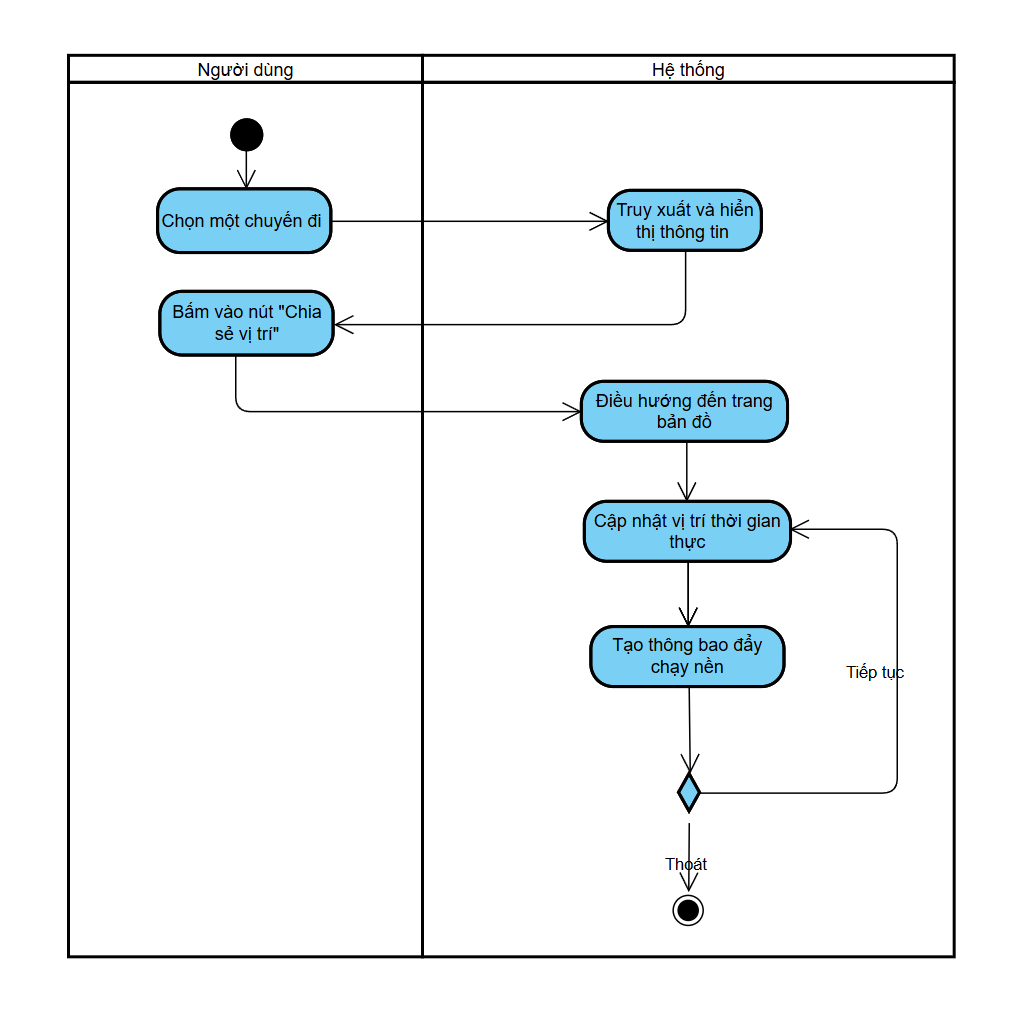
\includegraphics[width=0.5\linewidth]{figures/c3/3-3-16-ad.png} % Specified width
        &
        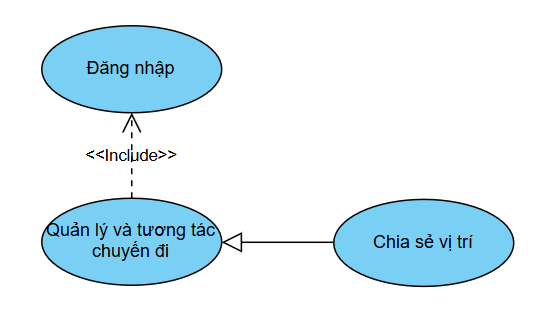
\includegraphics[width=0.45\linewidth]{figures/c3/3-3-16-rd.png} \\ % Specified width
        \hline
    \end{tabular}
\end{table}

\begin{figure}[H]
    \centering
    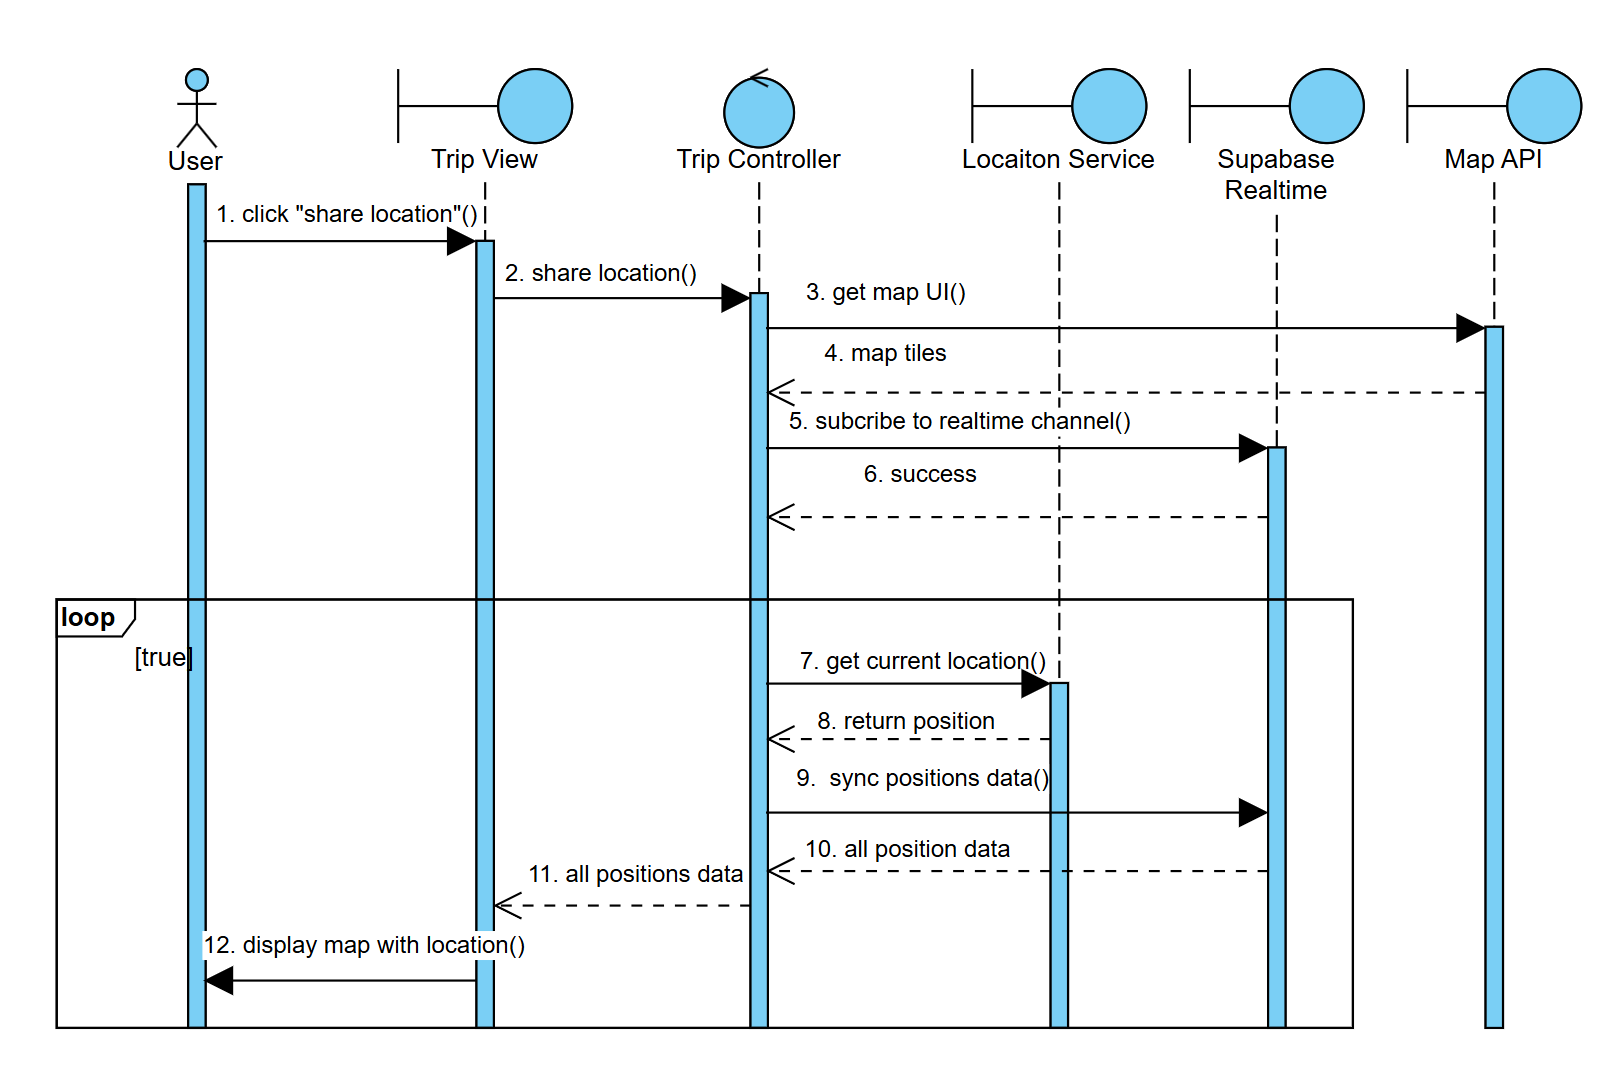
\includegraphics[width=1\textwidth]{figures/c3/3-3-16-sd.png} % Specified width
    \caption{Biểu đồ tuần tự ca sử dụng chia sẻ vị trí} % (no period)
    \label{fig:3-3-16-sequence-diagram}
\end{figure}
\nopagebreak
% \input{chapters/c3/usecases_details/3.3.17_uc}\nopagebreak